\documentclass[12pt,twoside]{book}

%Para listado de programas
\usepackage{listings}
\usepackage{color}

\definecolor{mygreen}{rgb}{0,0.5,0}
\definecolor{mygray}{rgb}{0.7,0.7,0.7}
\definecolor{mymauve}{rgb}{0.58,0,0.82}

\lstset{ %
	 backgroundcolor=\color{mygray},   % choose the background color; you must add \usepackage{color} or \usepackage{xcolor}
	 basicstyle=\footnotesize\ttfamily,        % the size of the fonts that are used for the code
	 breaklines=true,            % Zeilen werden Umgebrochen
	 keywordstyle=\color{red},
	 commentstyle=\itshape\color{mygreen},    % comment style
	 numbers=left,                    % where to put the line-numbers; possible values are (none, left, right)
	 numbersep=5pt                   % how far the line-numbers are from the code
}

%Paquete de Idioma
\usepackage[spanish]{babel}

%Codificación Alfabeto
\usepackage[utf8]{inputenc}

%Codificación de Fuente
\usepackage[T1]{fontenc}

%Índice
\usepackage{makeidx}

%Gráficos
\usepackage{graphicx}
\usepackage{float} 
%\usepackage{xcolor} 

%Matemática
\usepackage{amsmath}
\usepackage{amsfonts}
\usepackage{amssymb}
\usepackage{amstext} 

%Estilo de Página Numeración superior
%\pagestyle{headings}

%un estilo propio
\usepackage{fancyhdr}
\setlength{\headheight}{15pt}

\pagestyle{fancy}
\renewcommand{\chaptermark}[1]{ \markboth{\chaptername\ \thechapter: #1}{} }
\renewcommand{\sectionmark}[1]{ \markright{ Sección \thesection. #1}{} }

\fancyhf{}
\fancyhead[LE,RO]{\thepage}
\fancyhead[RE]{\textit{ \nouppercase{\leftmark}} }
\fancyhead[LO]{\textit{ \nouppercase{\rightmark}} }
\fancyfoot[CE]{\textit{\textcopyright 2015 Laboratorio de Sistemas Embebidos\\
	                    UPAEP} }
\fancyfoot[CO]{\textit{LSE003-2015 \\
		Elaboró: Dr. Casimiro Gómez González} }	            
\fancypagestyle{plain}{ %
	\fancyhf{} % remove everything
	\renewcommand{\headrulewidth}{0pt} % remove lines as well
	\renewcommand{\footrulewidth}{0pt}
}

%Hiperlinks \href{url}{text}
\usepackage[pdftex]{hyperref}

\usepackage{cite} % para contraer referencias

%Titulo
\title{LSE003-2015: Diseño de Sistemas Embebidos}
\author{Dr. Casimiro Gómez González\\
	Facultad de Electrónica, UPAEP\\
               correo: casimiro.gomez@upaep.mx\\
               Tel: 222 229 9428}
\date{Primavera 2015}

\begin{document}

\maketitle

\chapter*{Prólogo}

El presente material ha sido elaborado en el laboratorio de sistemas embebidos UPAEP, y se ha desarrollado con la experiencia de estudiantes y profesores que han colaborado en dicho laboratorio. Hay material propio de clases y otro material generado a través de proyectos de vinculación y consultaría. Cualquier comentario o corrección favor de enviarlo por correo al autor.

\begin{flushright}
	
	El autor\\
	Casimiro Gómez González\\
	Doctor en Ingeniería Mecatrónica \\
	correo: casimiro.gomez@upaep.mx
\end{flushright}

\tableofcontents


\chapter{Conceptos Básicos de Sistemas Embebidos}

Los últimos diez años mas o menos, el mundo de la computación se ha movido desde las máquinas de escritorio grandes y estáticas a los dispositivos embebidos pequeños y móviles. Sistemas de software corriendo en redes de móviles, y los dispositivos embebidos deben tener propiedades que no siempre requieren los sistemas tradicionales:
\begin{itemize}
	\item Rendimiento cerca del óptimo
	\item Robustez
	\item Distribución
	\item Dinamismo
	\item Movilidad
\end{itemize}

Una de las diferencias en la ingeniería de software para sistemas embebidos es el conocimiento adicional que el ingeniero tiene de potencia eléctrica y electrónica; interfaces físicas de electrónica analógica y digital con la computadora; y diseño de software para sistemas embebidos y procesamiento digital de señales.

Cerca del 95\% de los sistemas de software son actualmente embebidos. Considera los dispositivos que tienes en casa de uso diario:

\begin{itemize}
	\item Teléfono Celular, iPOD, microondas
	\item receptor satelital de TV, receptor de TV de cable
	\item Unidad de control de automovil
	\item Reproductor de DVD
\end{itemize}

El desarrollo de software embebido usa los mismos modelos de desarrollo de software que las otras técnicas convencionales, incluyendo el modelo \textit{Waterfall}, el modelo en \textit{espiral} y el modelo \textit{Agile}.

\begin{figure}
	\centering
	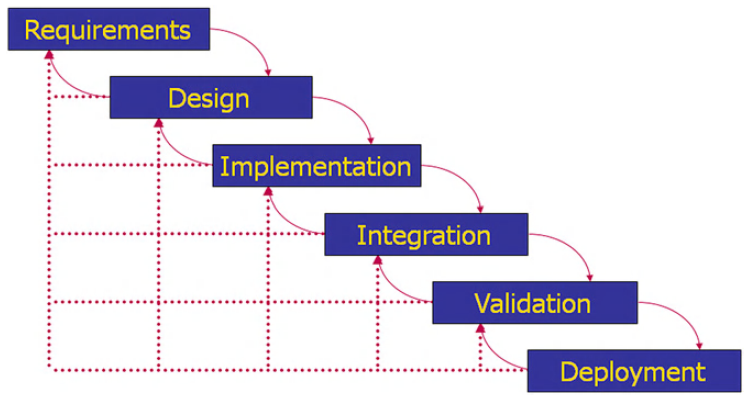
\includegraphics[width=0.9\linewidth]{waterfall.png}
	\caption{Modelo de desarrollo de software \textit{Waterfall}}
	\label{fig0001}
\end{figure}

\begin{figure}
	\centering
	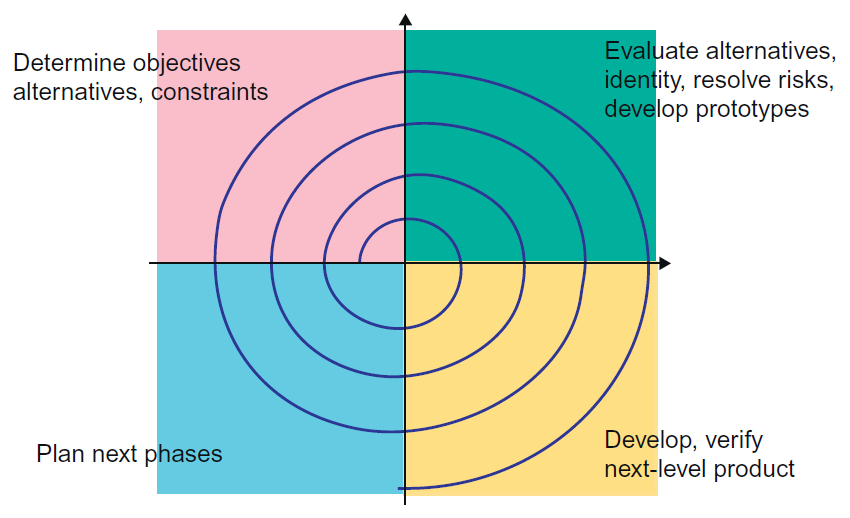
\includegraphics[width=0.9\linewidth]{espiral.png}
	\caption{Modelo de desarrollo de software \textit{Espiral}}
	\label{fig0002}
\end{figure}

\begin{figure}
	\centering
	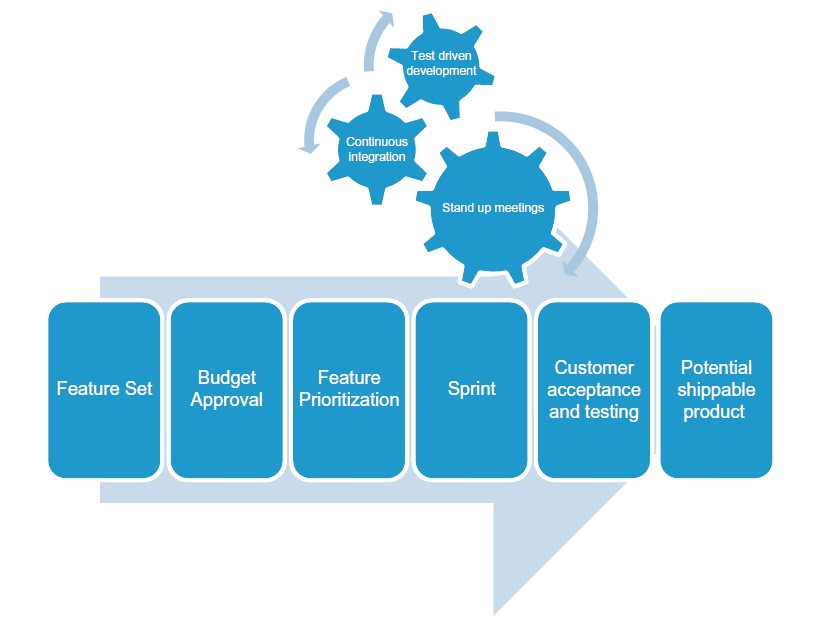
\includegraphics[width=0.9\linewidth]{agile.png}
	\caption{Modelo de desarrollo de software \textit{Agile}}
	\label{fig0003}
\end{figure}

La fases principales para el desarrollo de sistemas embebidos se pueden describir:
\begin{enumerate}
	\item \textbf{Definición del problema}: En esta fase se determina exactamente que quiere el cliente y el usuario. Esto incluye el desarrollo de un contrato con el cliente, dependiendo que tipo de producto esta siendo desarrollado. El objetivo de esta fase es especificar que producto de software se hará. Las dificultades incluyen: la solicitud del cliente por el producto incorrecto, el cliente no sabe sobre computación/software, lo cual limita la efectividad de esta fase, las especificaciones por lo regular son ambiguas, inconsistentes e incompletas.
	\item \textbf{Arquitectura/diseño}: La arquitectura se refiere a la selección de los elementos de arquitectónicos, sus interacciones, y las restricciones de aquellos elementos y sus interacciones necesarios para proporcionar un ambiente de trabajo con el cual satisfacer los requerimientos y servir como base para el diseño.  El diseño se refiere a la modularización y detalle de interfaz entre los elementos de diseño, sus algoritmos y procedimientos, y los tipos de datos necesarios para soportar la arquitectura y satisfacer los requerimientos. Durante la fase de arquitectura y diseño, el sistema es descompuesto en módulos de software con interfaces. Durante el diseño, el equipo de software desarrolla las especificaciones de los módulos (algoritmos y los tipos de datos),  manteniendo un récord de las decisiones de diseño y la trazabilidad, y especifica como los productos de software harán estas tareas. La dificultad principal durante esta fase incluye la falta de comunicación entre los diseñadores de módulos y terminan desarrollando un diseño que puede ser inconsistente, incompleto y ambiguo.
	\item \textbf{Implementación}: Durante esta fase el equipo de desarrollo implementa los módulos y componentes y verifica que cumplan las especificaciones. Los módulos se combinan de acuerdo con el diseño. Las implementaciones especifican como los productos del software hacen su trabajo. Algunas de las dificultades principales incluyen los errores de interacción entre los módulos y los errores de integración que pueden influenciar la calidad y la productividad.

	\item \textbf{Verificación y Validación(V\&V)}: Hay varias formas de V\&V. Una forma es el ``análisis''. El análisis puede ser en la forma de verificación estática, científica y fromal y en revisiones informales. Las pruebas es una forma dinámica de V\&V. Esta froma de pruebas viene en la froma de una caja blanca (se tiene acceso al código) y de caja negra (no hay acceso al código). Las pruebas pueden ser estructurales o de comportamiento.Hay pruebas estandares para realizar dependiendo del producto a desarrollar.
	 
\end{enumerate}

Mas y mas desarrollo de software para sistemas embebidos se esta moviendo al desarrollo basado en componentes.Este tipo de desarrollo es aplicado generalmente para componentes de tamaño razonable y reutilización a través del sistema, que es una tendencia creciente en sistemas embebidos. Los desarrolladores aseguran que estos componentes son adaptables a contextos variantes y extienden la idea mas alla del código a otros artefactos desarrollados tambien. Esta ténica cambia la ecuación desde ``Integración, entonces Bajar al Hardware'' a ``Bajar al Hardware, entonces Implementar''.

\chapter{Configurando las herramientas}

Aún cuando muchas de las técnicas de programación para las tarjetas embebidas se realizan en Python, el hecho de que es un lenguaje interpretado provoca que muchas de las aplicaciones desarrolladas en este lenguaje sean mucho mas lentas que las desarrolladas en lenguajes compilados como C. Este problema es principalmente crítico para proyectos con aplicaciones gráficas o procesamiento gráfico. Una solución es utilizar un lenguaje que tenga la rapidez de C y la facilidad de programación de Python, la propuesta en el lenguaje Vala, con un enfoque moderno de programación orientada a objetos.



\section{Instalando GTK+}

Lo primero que debemos instalar es el software GTK+, para ello se ejecuta desde la terminal:
\begin{lstlisting}[language=bash]
sudo apt-get install libgtk-3-dev
\end{lstlisting}

Si te marca un error al instalar esta librería entonces realizar los siguientes pasos:

\begin{lstlisting}[language=bash]
sudo apt-get install aptitude
sudo aptitude install libgtk-3-div
\end{lstlisting}


\section{Compartiendo Internet}

En el directorio /boot editar el archivo cmdline.txt y al final de la línea poner:
ip=ip de la rasp:: ip de la computadora : máscara de subred :rpi:eth0:off

En mi caso ha sido
ip=192.168.137.2::192.168.137.1:255.255.255.0:rpi:eth0:off


\section{Instalando Anjuta como IDE de programación en Vala}

Debido a que los proyectos que se realizarán serán en dos plataformas de programación, Vala y Python, el IDE que trabaja con ambos de manera muy eficiente se llama Anjuta. Y es este IDE el que se instalará. 

\subsection{Instalación de Vala}

Para instalar vala en Ubuntu se debe ejecutar el siguiente comando:

\begin{lstlisting}[language=bash]
sudo apt-get install valac
\end{lstlisting}

\subsection{Pasos para instalar Anjuta en Ubuntu}

Para instalar Anjuta para el lenguaje Vala y Python 3 debe seguirse los siguientes pasos:

\subsubsection{Primer paso}
Desde una terminal ejecutar:
\begin{lstlisting}[language=bash]
sudo apt-get install anjuta anjuta-extras 
sudo apt-get install python3 python3-pkg-resources
\end{lstlisting}

\subsubsection{Segundo Paso}

Bajar la última versión de python3. Y desde https://pypi.python.org/pypi/rope\_py3k bajar la ultima versión de Rope ( en esta caso rope\_py3k-0.9.4-1.tar.gz). Una vez bajado el archivo tenemos que abrir una terminal en la carpeta donde se encuentra y allí ejecutar lo siguiente:

\begin{lstlisting}[language=bash]
tar zxvf rope_py3k-0.9.4-1.tar.gz
cd rope_py3k-0.9.4-1/
sudo python3 setup.py install --prefix=/usr --install-lib=/usr/lib/python3/dist-packages
sudo ln /usr/lib/python3/dist-packages/rope_py3k-0.9.4_1-py3.4.egg-info /usr/lib/python3/dist-packages/rope-0.9.4_1-py3.4.egg-info
\end{lstlisting}

\subsubsection{Tercer Paso}

Ahora abrir una terminal y ejecutar python3. En la linea de comandos de Python3 checar si las siguientes instrucciones no marcan ningún error. De marcar algún error revisar los pasos anteriores.

\begin{lstlisting}[language=Python]
import rope
import pkg_resources
pkg_resources.get_distribution('rope').version 
\end{lstlisting}

\subsubsection{Cuarto Paso}

Ahora hay que corregir el archivo script de Anjuta para poder ejecutar Python3 

\begin{lstlisting}[language=bash]
sudo nano /usr/lib/anjuta/anjuta-python-autocomplete.py
\end{lstlisting}

agregando al principio de este archivo la siguiente linea 

\begin{lstlisting}[language=Python]
from __future__ import print_function
\end{lstlisting}


Entonces modifica todos los comandos  \textbf{print blahblah} a la sintaxis de python3: \textbf{print(blahblah)}, los comandos \textbf{print} estan en las lineas 124, 143 y 144.
Ahora inicia Anjuta y seleccionando \textbf{Edit->Preferences->Python->Environment}: cambiar el compilador a: \textbf{/usr/bin/python3}.   

\section*{Errores comunes}

Una vez instalado Anjuta es posible que al compilar el primer proyecto, marque un error de las librerías \textbf{libtool}, por lo regular estas librerías se instalan junto con el Anjuta. Sin embargo, la dependencia no es con respecto a las librerías sino con respecto a los binarios de dichas librerias, por lo tanto para instalarlo es necesario ejecutar:

\begin{lstlisting}[language=bash]
sudo apt-get install libtool-bin
\end{lstlisting}

Una vez instalados los binarios de la librería, con el comando anterior, el problema se resuelve.
\section{¿Que es Vala?}
Vala es un nuevo lenguaje de programación que permite usar técnicas de programación modernas para desarrollar aplicaciones que se ejecutan usando las bibliotecas de GNOME, aunque también es posible ejecutarlo en otros sistemas operativos y entornos gráficos, debido a sus bajas dependencias (GLib y GObject). Esta plataforma de desarrollo provee de un entorno completo de programación; con funcionalidades como el sistema de tipos dinámicos y el gestor de memoria asistida. Antes de la existencia de Vala, la única forma de programar para la plataforma era con la API nativa de C, o utilizando un lenguaje de programación de alto nivel que usan máquinas virtuales, como Python o C\#, que necesitan un wrapper para usar esa biblioteca.


Vala es un lenguaje totalmente diferente de otros lenguajes y otras técnicas, ya que el compilador genera código en lenguaje C, que puede ser compilado para ser ejecutado sin ninguna biblioteca extra ni wrapper intermedio. Esto tiene una serie de consecuencias, pero entre las mas importantes se encuentran:

\begin{enumerate}
	\item Los programas escritos en Vala debería tener un desempeño similar al mismo programa directamente escrito en lenguaje C. Siendo mucho más fácil y rápido de escribir y mantener.
	\item Una aplicación escrita en Vala no puede hacer nada que un programa equivalente escrito en lenguaje C no pueda hacer. Sin embargo Vala introduce una serie de funcionalidades que no están disponibles en C, las cuales se mapean en construcciones escritas en C, siendo estas últimas difíciles y complejas de escribir directamente.
\end{enumerate}

Vala es, por lo tanto, un lenguaje de programación moderno con todas las funcionalidades que se puede esperar de una plataforma actual (Python, .NET, etc).

Vala comparte bastante sintaxis con C\#, pero algunas otras no se corresponden con construcciones de este lenguaje, por tanto no se entrará en comparación a menos que sea necesario, para evitar que este libro esté enfocado a programadores de C\#.

 Es importante darse cuenta que Vala realmente se ejecuta como un programa escrito en C compilado, y puede interactuar con bibliotecas escritas en C. Por tanto un conocimiento de C puede hacer comprender el funcionamiento de Vala.

\section{Primer Programa de Vala}

El primer programa en Vala va a ser el conocido como "Hola Mundo" que es el programa más simple (sin contar con el programa vacío) que se puede escribir en un lenguaje de programación.

El listado de código sería algo como lo que sigue:

\begin{lstlisting}[language=C++]
class Demo.HelloWorld : GLib.Object {
	public static int main(string[] args) {
		stdout.printf("Hola, mundo!\n");
		return 0;
	}
}
\end{lstlisting}


 La primera línea que se ve es:
\begin{lstlisting}[language=C++]
class Demo.HelloWorld : GLib.Object {
\end{lstlisting}

Esta línea de código representa la definición de una nueva clase llamada HelloWorld. Se puede observar que antes del nombre de la clase se encuentra la palabra ``Demo'' seguida de un punto. Bien, esto indica el espacio de nombres en el que se mueve el programa. Asimismo, se puede observar que después del nombre de la nueva clase le siguen dos puntos y la cadena ``Glib.Object''. Esta cadena va en el mismo formato que la anterior, es decir, ``espacio de nombres''.``nombre de la clase'' e indica una clase de la que hereda la clase anterior. La mayoría de las nuevas clases heredarán de la clase ``GLib.Object'' que puede ser considerada como la clase básica en el lenguaje Vala, ya que, una parte importante de las funcionalidades del lenguaje están supeditadas a que la clase sobre las que se aplican hereden de esta clase o de una clase descendiente de ésta. Como se ha podido ver la sintaxis de definición de una clase es bastante similar a otros lenguajes de programación como C++, Java o C\#.

Siguiendo con el mismo listado de código tenemos que la siguiente línea de código es la que sigue a continuación:

\begin{lstlisting}[language=C++]
public static int main(string[] args) {
\end{lstlisting}

Esta línea de código define un método de la clase HelloWorld llamado ``main''. Este método va precedido por la palabra reservada ``public'' que indica que se trata de un método público (es decir, puede ser llamado externamente a la clase a la que pertenece). La palabra reservada ``static'' nos indica que se trata de un método estático (está asociado a la clase y no a un objeto en concreto, es decir, puede ser llamado sin instanciar ningún objeto de esa clase). Además se indica que el tipo de datos que devuelve este método es de tipo entero, lo que se hace mediante la palabra reservada ``int''. Por último, entre los paréntesis se indican los parámetros (los datos que utilizará internamente el método para trabajar). El parámetro es una lista de cadenas que contendrá los parámetros con los que fue llamado el programa desde la línea de comandos. El hecho de que el método definido se llame ``main'' no es casual, ya que, Vala considera a este método concreto como el punto de entrada del programa, es decir, que una vez compilado un programa escrito en Vala éste será el primer método en ser ejecutado. Este método es el que contiene la correspondientes inicializaciones que requiere el programa que estemos desarrollando, por ejemplo la inicialización de la interfaz gráfica de usuario.

\begin{lstlisting}[language=C++]
stdout.printf("Hola, mundo!\n");
\end{lstlisting}
Esta línea de código imprime por la salida estándar (normalmente será la pantalla del ordenador) el mensaje encerrado entre comillas. Es una llamada al método ``printf'' del objeto ``stdout''. En el lenguaje de programación Vala existen una serie de objetos predefinidos a los cuales tenemos acceso por que se encuentran definidos dentro del espacio de nombres GLib que está definido por defecto en cualquier programa Vala. El objeto ``stdout'' nos permite el acceso a la salida estándar de la máquina y entre otros métodos contiene el método ``printf'' que muestra un mensaje formateado por dicha salida.

La última línea importante del código inicial es la siguiente:

\begin{lstlisting}[language=C++]
return 0;
\end{lstlisting}
 
 Esta línea hace que el programa finalice y devuelva un valor de 0 al sistema. Este valor normalmente se usa para indicar si un programa ha finalizado de forma correcta o no. Si estuviera definido en otro método cualquiera (que no fuera el punto de entrada del programa) devolvería el valor y se almacenaría en una variable. Por ejemplo:
 
\begin{lstlisting}[language=C++]
int valor = objeto.metodo();
\end{lstlisting}
 
 
 Las últimas líneas del listado únicamente cierran la definición de la clase y el método definido como en cualquier otro lenguaje como por ejemplo C++ o Java.
 
 \section{Compilación del programa en Vala}
 
  El siguiente paso es compilar dicho programa. Vala al ser un lenguaje de programación compilado y por lo tanto necesita de un compilador. El lenguaje de programación Vala dispone de un compilador llamado ``valac'' y que es compilador al mismo tiempo del lenguaje de programación Genie.
  
  Asumiendo que tenemos el compilador de Vala instalado en nuestra máquina, para compilar el primer programa ``Hola mundo'' suponiendo que está escrito en un fichero llamado ``hola.vala'' sería:

\begin{lstlisting}[language=bash]
valac hola.vala
\end{lstlisting}
 
 Esto generaría un fichero ejecutable llamada ``hola'' (dependiendo del sistema operativo en el que nos encontremos el fichero binario resultante tendrá o no una extensión como por ejemplo la ``.exe'' en Windows). Para ejecutar dicho programa habrá que escribir en la línea de comandos algo como:
 
\begin{lstlisting}
./hola
\end{lstlisting}
 
 Y nos mostrará la salida:
 
\begin{lstlisting}[language=bash]
 Hola, mundo!
\end{lstlisting}
 
 Los archivos de código fuente de vala tienen, normalmente, la extensión ``.vala''. El lenguaje de programación Vala no fuerza a que los proyectos tengan una determinada estructura, en cuanto a los paquetes o los nombres de los archivos que contiene una clase, como hacen otros lenguajes como Java. En lugar de eso la estructura se define dentro de los archivos de código mediante texto, definiendo la localización y estructura lógica mediante elementos como los espacios de nombres. Cuando se quiere compilar código Vala, se le pasa al compilador una lista de los archivos de código fuente necesarios, y el compilador determina como ensamblarlos todos juntos.
 
 La ventaja de todo esto es que se pueden definir tantas clases o funciones como se desee dentro de un único archivo de código, incluso combinando distintos espacios de nombres todos dentro del mismo archivo (aunque no se demasiado recomendable por cuestiones de legibilidad y estructura). Vala por lo tanto no exige de manera inherente una determinada estructura para los proyectos que se desarrollan usando esta plataforma. Sin embargo, si existen ciertas convenciones a la hora de estructurar un proyecto desarrollado en Vala. Un buen ejemplo sería como se estructura el propio proyecto del compilador de Vala.
 
 Todos los archivos de código que pertenezcan al mismo proyecto son suministrados al compilador ``valac'' mediante la línea de comandos, junto con los correspondientes parámetros de compilación. Esto funciona de forma similar a como se haría con el código fuente compilado en Java. Por ejemplo:

\begin{lstlisting}[language=bash]
$ valac compiler.vala --pkg libvala
\end{lstlisting} 

Esa línea de código produciría un archivo binario llamado "compiler" que sería enlazado con el paquete "libvala" (cuando nos referimos a paquete lo estamos haciendo a un concepto similar a biblioteca de funciones o la mal traducida librería). De hecho, así es como se genera el compilador de Vala en realidad.

Si se quiere que el archivo ejecutable producido tenga un nombre específico (distinto al que el compilador le da) o si se le pasan varios archivos al compilador, es posible especificar el nombre del fichero ejecutable mediante la opción ``-o'':

\begin{lstlisting}[language=bash]
$ valac source1.vala source2.vala -o myprogram
$ ./myprogram
\end{lstlisting}

Como se ha comentado anteriormente el compilador de vala es capaz de generar código en lenguaje C en lugar de un archivo ejecutable. Así para realizar esto existe la opción ``-C'' que indicará al compilador que genere todo el código C necesario para crear el ejecutable del proyecto. El compilador creará un archivo con extensión ``.c'' por cada archivo con extensión ``.vala'' que le pasemos. Si abrimos el contenido de esos archivos generados se puede ver el código C equivalente al programa que hemos desarrollado en Vala. Se puede observar como se crean las mismas clases que en Vala pero mediante la biblioteca GObject y cómo se registran de forma dinámica en el sistema. Este es un ejemplo del poder que tiene la plataforma de desarrollo de GNOME. Sin embargo, todo esto es a título informativo, ya que, por suerte no es necesario generar todos estos ficheros, ni entender como funcionan internamente para poder programar en Vala. Si en lugar de generar el fichero de código C sólo necesitamos generar la cabecera (por ejemplo si estamos generando una biblioteca de funciones será necesario para poder usarla en C o en otro lenguaje) existe la opción ``-H'' con la que conseguiremos ese objetivo. A continuación un ejemplo que genera los dos ficheros (un fichero de código C y su correspondiente cabecera ``.h''):

\begin{lstlisting}[language=bash]
$ valac hello.vala -C -H hello.h
\end{lstlisting}
 
\chapter{Configurando FreeBSD}

\section{Cambiar idioma al español}
En la carpeta local de los usuarios (esta carpeta se encuentra en /usr/home/TU\_USUARIO).

\begin{lstlisting}[language=bash]
ee .login_conf

me:
:charset=ISO-8859-15:
:lang=es_ES.ISO8859-15:
:tc=default:
\end{lstlisting}



Ahora se configura el archivo .profile

\begin{lstlisting}[language=bash]
ee .profile

LANG=es_ES.ISO8859-15; export LANG
MM_CHARSET=ISO-8859-15; export MM_CHARSET
\end{lstlisting}

Se configura el archivo de inicio de xwindows

\begin{lstlisting}[language=bash]
ee .xinitrc

LANG=es_ES.ISO8859-15; export LANG
setenv LANG es_ES.ISO8859-15
\end{lstlisting}

\section{Como instalar Xwindows en freebsd para ARM}
Para la instalación de Xwindows en la tarjeta embebida con FreeBSD es necesario instalar los controladores primero:

\begin{lstlisting}[language=bash]
# pkg install xf86-video-scfb xf86-video-fbdev
# pkg install xorg
\end{lstlisting}

Crear el archivo xorg.conf ejecutando el comando: 

\begin{lstlisting}[language=bash]
ee /etc/X11/xorg.conf
\end{lstlisting}

y capturar el siguiente código:

\begin{lstlisting}[language=bash]
Section "Device"
Identifier "Generic FB"
Driver "scfb"
EndSection

Section "Screen"
Identifier "Screen"
Device "Generic FB"
Monitor "Monitor"
SubSection "Display"
Depth 16 #24 #32
EndSubsection
EndSection
\end{lstlisting}

Una vez configurado XWINDOWS se ejecuta con el comando:

\begin{lstlisting}[language=bash]
#startx 
\end{lstlisting}

Para instalar el ambiente de escritorio MATE se ejecuta el siguiente comando:
 
\begin{lstlisting}[language=bash]
pkg install  mate-desktop mate 
\end{lstlisting}


para ejecutar MATE:

\begin{lstlisting}[language=bash]
xinit mate-session 
\end{lstlisting}

\chapter{Sintaxis de Vala}
La sintaxis de Vala es una mezcla, basada principalmente en la de C\#. Como resultado, la mayor parte de esta debería ser familiar para los programadores que conozcan cualquier lenguaje similar a C. Teniendo esto en cuenta, se hará una descripción breve de la misma.

El alcance de declaración se define mediante corchetes. Un objeto o referencia sólo es válido entre { y }. Estos delimitadores se usan también para definir clases, métodos, bloques de código, etc, de manera que tengan automáticamente su propio alcance. Vala no es estricto acerca de dónde se declaran las variables.

Un identificador se define por su tipo y nombre, por ejemplo, int c describe un entero llamado c. En el caso de los tipos por valor, esto también crea un objeto del tipo dado. Para tipos referenciados esto simplemente define una nueva referencia que no apunta a nada inicialmente.

Para los nombres de identificadores, se aplican las mismas reglas que para los identificadores de C: el primer carácter debe estar entre [a-z], [A-Z] o subrayados ( \_ ), los siguientes pueden estar entre estos y [0-9]. No se permiten otros caracteres Unicode. Es posible usar palabras reservadas como identificadores, añadiéndoles el carácter @ como prefijo. Este carácter no forma parte del nombre. Por ejemplo, puede llamar a un método foreach escribiendo @foreach, siendo esta una palabra reservada de Vala.

Los tipos por referencia se instancian empleando el operador new y el nombre de un método de construcción, que generalmente es el propio nombre del tipo, por ejemplo, \textbf{Object o = new Object()} crea un \textbf{Object} nuevo y convierte a o en una referencia a este.

\section{Comentarios}

Vala permite varias maneras de escribir comentarios en el código:
\begin{lstlisting}[language=C++]
// Los comentarios continuan hasta el final de la linea

/* Los comentarios estan entre los delimitadores*/

/**
* Comentarios de Documentos
*/
\end{lstlisting}

Estos comentarios se manejan de la misma manera que en la mayoría de lenguajes, y requieren por ello poca explicación. Los comentarios para documentación no son específicos de Vala, pero una herramienta de generación de documentación como Valadoc los reconoce.

\section{Tipos de datos}

En general, hay dos tipos de dato en Vala: \textbf{tipos referenciados} y \textbf{tipos por valor}. Estos nombres describen cómo se usan en el sistema las instancias de los tipos; un tipo por valor se copia cada vez que se asigna a un identificador nuevo, un tipo referenciado no se copia, en lugar de esto el nuevo identificador es una nueva referencia al mismo objeto.

Una constante se define poniendo \textbf{const} delante del tipo. El convenio para constantes es \textbf{TODO\_EN\_MAYUSCULAS}.

\section{Tipos por valor}

Vala soporta un conjunto de tipos simples, como la mayoría de lenguajes.

\begin{itemize}
	\item Byte: \textbf{ char, uchar}; sus nombres son char por motivos históricos.
	\item Carácter: \textbf{unichar}; un carácter Unicode de 32 bits.
	\item Entero: \textbf{int, uint}.
	\item Entero <<largo>>: \textbf{long,ulong}.
	\item Entero <<corto>>: \textbf{short, ushort}.
	\item Entero de tamaño garantizado: \textbf{int8, int16, int32, int64}, así como sus versiones sin signo \textbf{uint8, uint16, uint32, uint64}. Los números indican las longitudes en bits.
	\item Número real en coma flotante: \textbf{float, double}.
	\item Booleano, bool: sus valores posibles son \textbf{true (verdadero)} y \textbf{false (falso)}.
	\item Compuesto: \textbf{struct}.
	\item Enumerado: \textbf{enum}; representado por valores enteros, no por clases, como las enumerados de Java.
\end{itemize}

A continuación se muestran algunos ejemplos.

\begin{lstlisting}[language=C++]
/* Tipos Atomicos */
unichar c = 'u';
float percentile = 0.75f;
const double MU_BOHR = 927.400915E-26;
bool the_box_has_crashed = false;

/* Definiendo una estructura */
struct Vector {
	public double x;
	public double y;
	public double z;
}

/* Definiendo un enum */
enum WindowType {
	TOPLEVEL,
	POPUP
}
\end{lstlisting}

La mayoría de estos tipos pueden tener diferentes tamaños en distintas plataformas, exceptuando los tipos de tamaño garantizado. El operador \textbf{sizeof} devuelve el tamaño que ocupa, en bytes, una variable de un tipo dado:

\begin{lstlisting}[language=C++]
ulong nbytes = sizeof(int32); // nbytes will be 4 (= 32 bits)
\end{lstlisting}

Se pueden determinar los valores máximo y mínimo de un tipo numérico con \textbf{.MIN} y \textbf{.MAX}, por ejemplo, \textbf{int.MIN} e \textbf{int.MAX}.

\section{Cadena de Caracteres}

El tipo de dato para cadenas de caracteres es \textbf{string}. Las cadenas de Vala están codificadas en \textbf{UTF-8} y son inmutables.

\begin{lstlisting}[language=C++]
string text = "A string literal";
\end{lstlisting}

Vala ofrece una característica llamada cadenas literales (<<verbatim strings>>). Son cadenas de caracteres en las cuales las secuencias de escape (como puede ser \textbackslash n) no se interpretan, los saltos de línea se conservan y los signos de puntuación no tienen que enmascararse. Estas cadenas se delimitan con tres comillas dobles. Las posibles sangrías tras un salto de línea también forman parte de la cadena.

\begin{lstlisting}[language=C++]
string verbatim = """This is a so-called "verbatim string".
Verbatim strings don't process escape sequences, such as \n, \t, \\, etc.
They may contain quotes and may span multiple lines.""";
\end{lstlisting}

Las cadenas precedidas por @ son consideradas patrones. En ellas se evalúan las variables y expresiones precedidas por \$:

\begin{lstlisting}[language=C++]
int a = 6, b = 7;
string s = @"$a * $b = $(a * b)";  // => "6 * 7 = 42"
\end{lstlisting}

Los operadores de igualdad == y != comparan el contenido de dos cadenas de caracteres, a diferencia del comportamiento de Java, donde se compara la igualdad entre referencias.

Es posible dividir una cadena con [inicio:fin]. Los valores negativos representan posiciones relativas al final de la cadena:

\begin{lstlisting}[language=C++]
string greeting = "hello, world";
string s1 = greeting[7:12];        // => "world"
string s2 = greeting[-4:-2];       // => "or"
\end{lstlisting}

Obsérvese que los índices en Vala empiezan en 0 como en la mayoría de lenguajes de programación. Desde Vala 0.11 se puede acceder a un solo byte mediante [índice]:

\begin{lstlisting}[language=C++]
uint8 b = greeting[7];             // => 0x77
\end{lstlisting}

Sin embargo, no se puede asignar un byte nuevo a esta posición ya que, como se ha comentado anteriormente, las cadenas de caracteres en Vala son inmutables.

Muchos de los tipos básicos tienen métodos intuitivos para tomar el valor de una cadena, así como para convertir su valor a una cadena, por ejemplo:

\begin{lstlisting}[language=C++]
bool b = bool.parse("false");           // => false
int i = int.parse("-52");               // => -52
double d = double.parse("6.67428E-11"); // => 6.67428E-11
string s1 = true.to_string();           // => "true"
string s2 = 21.to_string();             // => "21"
\end{lstlisting}

Dos métodos útiles para escribir y leer cadenas en y desde la línea de comandos (y para las primeras pruebas con Vala) son, respectivamente, \textbf{stdout.printf()} y \textbf{stdin.read\_line()}:

\begin{lstlisting}[language=C++]
stdout.printf("Hello, world\n");
stdout.printf("%d %g %s\n", 42, 3.1415, "Vala");
string input = stdin.read_line();
int number = int.parse(stdin.read_line());
\end{lstlisting}

Ya se ha presentado \textbf{stdout.printf()} en el ejemplo HolaMundo. Este método acepta un número arbitrario de argumentos de distintos tipos, mientras que el primer argumento es una cadena de formato, que sigue las mismas reglas que las cadenas de formato de C. Si se requiere mostrar un mensaje de error, se puede emplear \textbf{\textit{stderr.printf()}} en lugar de \textbf{\textit{stdout.printf()}}.

Adicionalmente, la operación in puede utilizarse para determinar si una cadena contiene a otra, por ejemplo:

\begin{lstlisting}[language=C++]
if ("ere" in "Able was I ere I saw Elba.") ...
\end{lstlisting}


\section{Matrices}

Las matrices se declaran dando un nombre de tipo seguido de \textbf{[]} y se crean usando el operador \textbf{new}, por ejemplo, \textbf{int[]a = new int[10]} para crear una matriz de enteros. La longitud de estas matrices se puede obtener accediendo al miembro variable \textbf{length}, por ejemplo, \textbf{int count = a.length}. Se debe tener en cuenta que si se escribe \textbf{Object[] a = new Object[10]} no se creará ningún objeto, sólo la matriz para almacenarlos.

\begin{lstlisting}[language=C++]
int[] a = new int[10];
int[] b = { 2, 4, 6, 8 };
\end{lstlisting}

Una matriz se puede dividir con [inicio:fin]:

\begin{lstlisting}[language=C++]
int[] c = b[1:3];     // => { 4, 6 }
\end{lstlisting}

El resultado de dividir una matriz es una referencia a los datos requeridos, no una copia de estos. Sin embargo, si se asigna este resultado a una variable owned (como se ha hecho antes) sí que se copian los datos. Si se quiere evitar la copia, se puede optar por asignar el resultado a una matriz unowned o se puede pasar directamente a un argumento (los argumentos son, de manera predeterminada, unowned).

\begin{lstlisting}[language=C++]
unowned int[] c = b[1:3];     // => { 4, 6 }
\end{lstlisting}


Las matrices multidimensionales se definen con [,] o [,,], etc.

\begin{lstlisting}[language=C++]
int[,] c = new int[3,4];
int[,] d = {{2, 4, 6, 8},
	{3, 5, 7, 9},
	{1, 3, 5, 7}};
d[2,3] = 42;
\end{lstlisting}


Este tipo de matriz se representa como un bloque de memoria contigua. Las matrices multidimensionales compuestas ([][], también conocidas como ``matrices apiladas'' o ``matrices de matrices''), en las que cada fila puede tener diferente longitud, no están soportadas aún.

Para obtener la longitud de cada dimensión de una matriz multidimensional, el miembro length pasa a ser una matriz que almacena la longitud o cada dimensión respectivamente.

\begin{lstlisting}[language=C++]
int[,] arr = new int[4,5];
int r = arr.length[0];
int c = arr.length[1];
\end{lstlisting}

Tenga en cuenta que se no se pueden obtener una matriz de una dimensión a partir de una matriz multidimensional, ni siquiera dividir una matriz multidimensional:

\begin{lstlisting}[language=C++]
int[,] arr = {{1,2},
	{3,4}};
int[] b = arr[0];  // won't work
int[] c = arr[0,];  // won't work
int[] d = arr[:,0];  // won't work
int[] e = arr[0:1,0];  // won't work
int[,] f = arr[0:1,0:1];  // won't work
\end{lstlisting}

Se pueden añadir elementos a una matriz dinámicamente haciendo uso del operador +=. Sin embargo, sólo funciona para las matrices definidas localmente o privadas. La matriz se reubica automáticamente si es necesario. Internamente esta reubicación se realiza con tamaños crecientes en potencias de 2 por razones de eficiencia en tiempo de ejecución. No obstante, .length contiene el número actual de elementos, no el tamaño interno.

\begin{lstlisting}[language=C++]
int[] e = {};
e += 12;
e += 5;
e += 37;
\end{lstlisting}

El tamaño de una matriz se puede variar llamando a resize() sobre esta. Esta operación mantiene el contenido original (tanto de éste como quepa en el nuevo tamaño).

\begin{lstlisting}[language=C++]
int[] a = new int[5];
a.resize(12);
\end{lstlisting}

Si se ponen corchetes después del identificador junto a una indicación de tamaño, se creará una matriz de tamaño fijo. Las matrices de tamaño fijo se almacenan en la pila (si se usan como variables locales) o se almacenan in-line (si se usan como campos) y no se pueden reubicar más tarde.

\begin{lstlisting}[language=C++]
int f[10];     // no 'new ...'
\end{lstlisting}

Vala no comprueba los límites en tiempo de ejecución en el acceso a matrices. Si se requiere mayor seguridad, se debería usar una estructura de datos más sofisticada, como el ArrayList.

\section{Tipos referenciados}

Los tipos referenciados son todos los tipos declarados como una clase, independientemente de si descienden o no del Object de GLib. Vala se asegurará de que cuando se pasa un objeto por referencia el sistema mantenga la cuenta del número de referencias realizadas actualmente con el propósito de gestionar la memoria de forma automática. El valor de una referencia que no apunta a nada es null.

\begin{lstlisting}[language=C++]
/* defining a class */
class Track : GLib.Object {             /* subclassing 'GLib.Object' */
	public double mass;                 /* a public field */
	public double name { get; set; }    /* a public property */
	private bool terminated = false;    /* a private field */
	public void terminate() {           /* a public method */
		terminated = true;
	}
}
\end{lstlisting}

\section{Promoción de tipos estáticos}

En Vala es posible promocionar una variable de un tipo a otro. Para promocionar una variable de un tipo estático se escribe el tipo deseado entre paréntesis. La promoción estática no impone ningún tipo de comprobación de seguridad de los tipos en tiempo de ejecución. Funciona para todos los tipos disponibles en Vala. Por ejemplo:

\begin{lstlisting}[language=C++]
int i = 10;
float j = (float) i;
\end{lstlisting}

Vala soporta otro mecanismo de promoción llamado \textit{promoción dinámica} que realiza comprobación de tipos en tiempo de ejecución y se describe en la sección sobre programación orientada a objetos.

\section{Inferencia de Tipos}

Vala cuenta con un mecanismo llamado \textit{inferencia de tipos}, con la que una variable local se puede definir usando \textbf{\textit{var}} en vez de indicar un tipo, mientras que no haya ambigüedad en el tipo que se ha querido indicar. El tipo se infiere de la asignación del lado derecho del igual. Esto ayuda a reducir redundancia innecesaria en el código sin sacrificar el tipado estático:

\begin{lstlisting}[language=C++]
var p = new Person();     // same as: Person p = new Person();
var s = "hello";          // same as: string s = "hello";
var l = new List<int>();  // same as: List<int> l = new List<int>();
var i = 10;               // same as: int i = 10;
\end{lstlisting}

Este mecanismo sólo funciona para variables locales. La inferencia de tipos es especialmente útil para tipos con argumentos genéricos. Compare:

\begin{lstlisting}[language=C++]
MyFoo<string, MyBar<string, int>> foo = new MyFoo<string, MyBar<string, int>>();
\end{lstlisting}

frente a:
 
\begin{lstlisting}[language=C++] 
var foo = new MyFoo<string, MyBar<string, int>>();
\end{lstlisting} 
 

\section{Definir un tipo nuevo a partir de otro}

Definir un tipo nuevo significa derivarlo del que se necesite. Por ejemplo:

\begin{lstlisting}[language=C++] 
/* Define a new type from a container like GLib.List with elements type GLib.Value */
public class ValueList : GLib.List<GLib.Value> {
	[CCode (has_construct_function = false)]
	protected ValueList ();
	public static GLib.Type get_type ();
}
\end{lstlisting}

\section{Operadores}

\subsubsection{=}
Asignación. El operando de la izquierda debe ser un identificador, y el de la derecha un valor o referencia, según el caso.

\subsubsection{+, -, /, *, \%}

Aritmética básica, aplicada a los operandos izquierdo y derecho. El operador + también puede concatenar cadenas de caracteres.

\subsubsection{+=, -=, /=, *=, \%=}

Operaciones aritméticas entre los operandos izquierdo y derecho, donde el operando de la izquierda debe ser un identificador al que se asigna el resultado.

\subsubsection{++, --}

Operaciones de incremento y decremento con asignación implícita. Estos operandos sólo requieren un argumento, que debe ser un identificador de un tipo de dato simple. El valor se cambia y se asigna de nuevo al identificador. Estos operadores deben situarse como prefijo o como sufijo; en el primer caso el valor que se evalúe será el recién calculado, mientras que en el segundo caso se evaluará el valor original.

\subsubsection{|, \^{} , \&, ~, |=, \&=, \^{}=}

Operaciones a nivel de bit: disyunción (o ó ``or''), disyunción exclusiva (``xor''), conjunción (y o ``and'') y negación. Los operadores del segundo grupo incluyen asignación y son análogos a las versiones aritméticas. Todos estos operadores se pueden aplicar a cualquier tipo de dato simple. El hecho de que no exista un operador de asignación asociado a ~ se debe a que este es un operador unario. La operación equivalente es simplemente a = \~{}a.

\subsubsection{<<, >>}
Operaciones de desplazamiento de bits. Desplazan el operando de la izquierda un número de bits de acuerdo al operando de la derecha.

\subsubsection{$$<<=$$, $$>>=$$}

Operaciones de desplazamiento de bits. Desplazan el operando de la izquierda un número de bits de acuerdo al operando de la derecha. El operando de la izquierda debe ser un identificador, al que se asigna el resultado.

\subsubsection{==}

Comprobación de igualdad. Evalúa a un valor bool dependiendo de si los operandos izquierdo y derecho son iguales. En caso de los tipos por valor esto significa que los valores son iguales, en el caso de los tipos por referencia implica que los objetos sean la misma instancia. Una excepción a esta regla es el tipo string, que se evalúa según la igualdad del valor.

\subsubsection{<, >, >=, <=, !=}

Comprobaciones de desigualdad. Se evalua a un valor bool dependiendo de si los operandos izquierdo y derecho son distintos de la manera descrita en cada caso. Son validos para tipos por valor, y para el tipo string. En este último caso estos operadores compara orden lexicográfico.

\subsubsection{!, \&\&, ||}

Operaciones lógicas: negación (no), conjunción (y) y disyunción (o). Estos operadores se pueden aplicar a valores booleanos, requiriendo el primero un solo valor y los otros, dos valores.

\subsubsection{? :}

Operador condicional ternario. Evalúa una condición y devuelve el valor de la sub-expresión a la izquierda o a la derecha basándose en la veracidad de la condición: condición ? valor si es cierta : valor si es falsa.

\subsubsection{??}
Operador de comprobación de nulidad y asignación: a ?? b es equivalente a a != null ? a : b. Este operador es útil, por ejemplo, para asignar un valor predeterminado en caso de que una referencia sea nula:

\begin{lstlisting}[language=C++]
stdout.printf("Hello, %s!\n", name ?? "unknown person");
\end{lstlisting}


Comprueba si el operando de la derecha contiene al operando de la izquierda. este operador funciona en matrices, cadenas de caracteres, colecciones de datos o cualquier otro tipo que tenga un método contains() apropiado. Para cadenas puede realizar búsqueda de subcadenas.

Los operadores no se pueden sobrecargar en Vala. Hay operadores adicionales, válidos en el contexto de las declaraciones lambda y otras tareas específicas; estos se explicaran en el contexto en el que sean aplicables.



\subsubsection{in}
Comprueba si el operando de la derecha contiene al operando de la izquierda. este operador funciona en matrices, cadenas de caracteres, colecciones de datos o cualquier otro tipo que tenga un método contains() apropiado. Para cadenas puede realizar búsqueda de subcadenas.

Los operadores no se pueden sobrecargar en Vala. Hay operadores adicionales, válidos en el contexto de las declaraciones lambda y otras tareas específicas; estos se explicaran en el contexto en el que sean aplicables.

\section{Estructuras de Control}

A continuación se muestran varios ejemplos de código de diferentes estructuras de control y el efecto de dicho código:

\begin{lstlisting}[language=C++]
while (a > b) { a--; }
\end{lstlisting}

Decrementa a repetidamente, comprobando antes de cada iteración que a sea mayor que b.

\begin{lstlisting}[language=C++]
do { a--; } while (a > b);
\end{lstlisting}

Decrementa a repetidamente, comprobando después de cada iteración que a sea mayor que b.

\begin{lstlisting}[language=C++]
for (int a = 0; a < 10; a++) { stdout.printf("%d\n", a); }
\end{lstlisting}


Inicializa a a 0, después se imprime a repetidamente hasta que su valor deje de ser mayor de 10, el valor de a se incrementa tras cada iteración.

\begin{lstlisting}[language=C++]
foreach (int a in int_array) { stdout.printf("%d\n", a); }
\end{lstlisting}


Imprime en la salida cada entero de una matriz, o cualquier otra colección iterable. El significado de <<iterable>> se describirá más adelante.

Los cuatro tipos anteriores de bucle se pueden controlar con las palabras reservadas break y continue. Una instrucción break provocará que el bucle termine inmediatamente, mientras que continue saltará a la parte de la comprobación de la iteración (terminando así la iteración actual, pero sin salir del bucle).

\begin{lstlisting}[language=C++]
if (a > 0) { stdout.printf("a is greater than 0\n"); }
else if (a < 0) { stdout.printf("a is less than 0\n"); }
else { stdout.printf("a is equal to 0\n"); }
\end{lstlisting}

Ejecuta partes de código concretas dependiendo de un conjunto de condiciones. La primera condición que cumplir decide qué código se ejecuta, si a es mayor que 0 no se realizará la comprobación de si es menor que 0. Se permite cualquier cantidad de bloques else if, y uno o ningún bloque else.

\begin{lstlisting}[language=C++]
switch (a) {
	case 1:
	stdout.printf("one\n");
	break;
	case 2:
	case 3:
	stdout.printf("two or three\n");
	break;
	default:
	stdout.printf("unknown\n");
	break;
}
\end{lstlisting}

Una sentencia switch ejecuta exactamente una o ninguna sección de código basándose en el valor que se le pasa. En Vala no hay paso a través de los distintos casos (bloques etiquetados con la palabra reservada case), excepto en los casos vacíos. Para asegurar esto, cada case no vacío debe terminar con una de las palabras reservadas break, return o throw. Se pueden utilizar las sentencias switch con cadenas de caracteres.

Como nota para los programadores de C: las condiciones deben evaluarse siempre un valor booleano. Es decir, que si uno quiere comprobar si una variable es nula o 0, debe hacerlo explícitamente: if (object != null) \{ \} or if (number != 0) \{ \}.

\section{Elementos del lenguaje}

\subsection{Métodos}

En Vala, las funciones se llaman métodos, independientemente de si están definidas dentro de una clase o no. Desde este momento se empleará el término método.

\begin{lstlisting}[language=C++]
int method_name(int arg1, Object arg2) {
	return 1;
	}
\end{lstlisting}

El anterior fragmento de código define un método con el nombre method\_name, que toma dos argumentos, un entero y un Object (el primero pasado por valor y el segundo por referencia, como se ha descrito anteriormente). El método devuelve un entero, que en este caso es 1.

Todos los métodos Vala son funciones C, y por ello toman un numero arbitrario de argumentos y devuelven un valor (o ninguno si el método se declara como void). Se puede aproximar un mecanismo para devolver más valores, poniendo datos en lugares conocidos por el código que llama al método. Los detalles de este mecanismo se explicarán en la sección "Dirección de los parámetros", en la parte avanzada de este tutorial.

El convenio para los nombres de métodos en Vala es todo\_en\_minúscula con subrayados como separadores entre palabras. Este proceder puede parecer poco familiar a programadores de Java o C\#, acostumbrados a los nombres de métodos en CamelCase o mixedCamelCase. Pero con este estilo se consigue consistencia con otras bibliotecas de Vala y C/GObject.

No es posible tener varios métodos con el mismo nombre pero distinto prototipo dentro del mismo ámbito de definición (mecanismo conocido como ``sobrecarga de métodos''):

\begin{lstlisting}[language=C++]
void draw(string text) { }
void draw(Shape shape) { }  // not possible
\end{lstlisting}


Esto se debe al hecho de que se pretende que las librerías producidas con Vala puedan ser utilizadas también por programadores de C. En su lugar, en Vala se haría lo siguiente:

\begin{lstlisting}[language=C++]
void draw_text(string text) { }
void draw_shape(Shape shape) { }
\end{lstlisting}

Eligiendo nombres ligeramente distintos puede evitarse la colisión entre los nombres. En lenguajes que soportan sobrecarga de métodos, esta suele emplearse para ofrecer métodos de conveniencia con menos parámetros que enlazan con un método más general:

\begin{lstlisting}[language=C++]
void f(int x, string s, double z) { }
void f(int x, string s) { f(x, s, 0.5); }  // not possible
void f(int x) { f(x, "hello"); }           // not possible
\end{lstlisting}

En este caso puede usarse la característica predeterminada de los argumentos de Vala con el fin de conseguir un comportamiento parecido con un solo método. Pueden definirse valores por defecto para los últimos parámetros de un método, para evitar pasarlos explícitamente al llamar al método:


\begin{lstlisting}[language=C++]
void f(int x, string s = "hello", double z = 0.5) { }
\end{lstlisting}

Algunas llamadas posibles a este método podrían ser:

\begin{lstlisting}[language=C++]
f(2);
f(2, "hi");
f(2, "hi", 0.75);
\end{lstlisting}

Incluso se puede definir métodos con una lista de argumentos de longitud variable (varargs) como stdout.printf, aunque no es del todo recomendable. Más adelante se hablará de esto.

Vala realiza una comprobación de nulidad básica en los parámetros y los valores devueltos de los métodos. Si se permite que un parámetro o un valor de retorno sea null, el símbolo del tipo debe ir seguido con un modificador ?. Esta información adicional ayuda al compilador de Vala a realizar comprobaciones estáticas y añadir verificaciones en tiempo de ejecución en las precondiciones de los métodos, lo que puede ayudar a evitar errores relacionados como eliminar una referencia a un puntero a null.

\begin{lstlisting}[language=C++]
string? method_name(string? text, Foo? foo, Bar bar) {
	// ...
}
\end{lstlisting}

En este ejemplo text, foo y el valor de retorno pueden ser null, no obstante bar no debe ser null.

\section{Delegados}

\begin{lstlisting}[language=C++]
delegate void DelegateType(int a);
\end{lstlisting}

Los delegados (<<delegate>>) representan métodos, permitiendo que se puedan pasar fragmentos de código entre objetos. En el ejemplo de arriba se define un tipo llamado DelegateType que representa métodos que toman un int y no devuelven nada. Cualquier método que concuerde con este prototipo puede asignarse a una variable de este tipo o pasarse como un argumento de este tipo a un método.
\begin{lstlisting}[language=C++]
delegate void DelegateType(int a);

void f1(int a) {
	stdout.printf("%d\n", a);
}

void f2(DelegateType d, int a) {
	d(a);       // Calling a delegate
}

void main() {
	f2(f1, 5);  // Passing a method as delegate argument to another method
}
\end{lstlisting}


En este código se ejecuta el método f2, pasándole una referencia al método f1 y el número 5. f2 ejecutará entonces el método f1, pasándole a este el número.

Los delegados también pueden crearse localmente. Un método miembro de una clase puede asignarse a un delegado, por ejemplo:


\begin{lstlisting}[language=C++]
class Foo {
	
	public void f1(int a) {
		stdout.printf("a = %d\n", a);
	}
	
	delegate void DelegateType(int a);
	
	public static int main(string[] args) {
		Foo foo = new Foo();
		DelegateType d1 = foo.f1;
		d1(10);
		return 0;
	}
}
\end{lstlisting}

\section{Métodos anónimos o clausuras}

\begin{lstlisting}[language=C++]
(a) => { stdout.printf("%d\n", a); }
\end{lstlisting}

Un método anónimo, también conocido como expresión lambda, función literal o clausura, puede definirse en Vala con el operador =>. La lista de parámetros se sitúa al lado izquierdo del operador, mientras que el cuerpo del método va en el lado derecho.

Un método anónimo por sí mismo, como el del ejemplo de arriba, no tiene mucho sentido. Estos métodos sólo son útiles si se asignan directamente a una variable de un tipo delegado o si se pasan como argumento a otro método.

Tenga en cuenta que ni los tipos de los parámetros ni los del valor de retorno se indican explícitamente. En lugar de esto, los tipos se infieren del prototipo del delegado con el que se utilizan.

A continuación se muestra un ejemplo de asignación de un método anónimo a una variable delegada:

\begin{lstlisting}[language=C++]
delegate void PrintIntFunc(int a);

void main() {
	PrintIntFunc p1 = (a) => { stdout.printf("%d\n", a); };
		p1(10);
		
		// Curly braces are optional if the body contains only one statement:
		PrintIntFunc p2 = (a) => stdout.printf("%d\n", a);
		p2(20):
	}
\end{lstlisting}

Y seguidamente el paso de un método anónimo a otro método:

\begin{lstlisting}[language=C++]
delegate int Comparator(int a, int b);

void my_sorting_algorithm(int[] data, Comparator compare) {
	// ... 'compare' is called somewhere in here ...
}

void main() {
	int[] data = { 3, 9, 2, 7, 5 };
	// An anonymous method is passed as the second argument:
	my_sorting_algorithm(data, (a, b) => {
		if (a < b) return -1;
		if (a > b) return 1;
		return 0;
	});
}
\end{lstlisting}

Los métodos anónimos son verdaderas clausuras. Esto significa que se puede acceder a las variables locales del método externo desde el interior de la expresión lambda:

\begin{lstlisting}[language=C++]
delegate int IntOperation(int i);

IntOperation curried_add(int a) {
	return (b) => a + b;  // 'a' is an outer variable
}

void main() {
	stdout.printf("2 + 4 = %d\n", curried_add(2)(4));
}
\end{lstlisting}

En este ejemplo, curried\_add (consulte Currificación) devuelve un método recién creado que conserva el valor de a. El método devuelto se llama directamente más adelante con 4 como argumento, dando como resultado la suma de los dos números.


\section{Espacios de Nombres}

\begin{lstlisting}[language=C++]
namespace NameSpaceName {
	// ...
}
\end{lstlisting}

Todo lo que se encuentra entre las llaves en el código anterior está dentro del espacio de nombres \textbf{NameSpaceName} y se debe hacer referencia a ello como tal. Cualquier fragmento de código fuera de este espacio de nombres, deberá usar nombres completos para acceder a todo lo que se encuentra dentro, o bien estar situado en un archivo con la declaración \textbf{using} adecuada para importar este espacio de nombres:

\begin{lstlisting}[language=C++]
using NameSpaceName;

// ...
\end{lstlisting}

Por ejemplo si el espacio de nombres Gtk se importa con \textbf{using Gtk;} se puede escribir simplemente Window en lugar de \textbf{Gtk.Window}. Un nombre completo sólo será necesario en caso de ambigüedad, por ejemplo entre \textbf{GLib.Object} y \textbf{Gtk.Object}.

El espacio de nombres \textbf{GLib} se importa de manera predeterminada. Imagine una línea \textbf{using GLib;} al principio de cada archivo Vala.

Todo lo que no se encuentre dentro de un espacio de nombres separado, quedará en el espacio de nombres anónimo global. Si se debe hacer referencia al espacio global explícitamente debido a una ambigüedad, puede hacerse usando el prefijo \textbf{global::}.

Los espacios de nombres puede estar anidados, bien anidando sus declaraciones o bien dando un nombre del tipo \textbf{NameSpace1.NameSpace2}.

Muchas otras definiciones pueden declararse dentro de un espacio de nombres siguiendo el mismo convenio, por ejemplo \textbf{class} \textbf{NameSpace1.Test { ... }}. Tenga en cuenta que cuando se hace esto el nombre final de la definición será aquel en el cual esté anidada la declaración más el espacio de nombre declarado en la definición.

\section{Struct}

\begin{lstlisting}[language=C++]
struct StructName {
	public int a;
}
\end{lstlisting}

El código presentado arriba define un tipo de \textbf{struct} (o estructura), es decir, un tipo de valor compuesto. Una estructura Vala puede contener métodos con ciertas limitaciones así como miembros privados, dado lo cual se requiere el modificador de acceso \textbf{public}.

\begin{lstlisting}[language=C++]
struct Color {
	public double red;
	public double green;
	public double blue;
}
\end{lstlisting}

De la siguiente manera se puede inicializar una estructura:

\begin{lstlisting}[language=C++]
// without type inference
Color c1 = Color();
Color c2 = { 0.5, 0.5, 1.0 };
Color c3 = Color() {
	red = 0.5,
	green = 0.5,
	blue = 1.0
};

// with type inference
var c4 = Color();
var c5 = Color() {
	red = 0.5,
	green = 0.5,
	blue = 1.0
};
\end{lstlisting}

Las estructuras se almacenan en la pila (<<stack>>) y se copian al asignarlas.

\section{Clases}

\begin{lstlisting}[language=C++]
class ClassName : SuperClassName, InterfaceName {
}
\end{lstlisting}

Este ejemplo define una clase, es decir un tipo por referencia. En contraposición a las estructuras, las instancias de las clases se almacenan en el montón (<<heap>>). Hay mucha más sintaxis relacionada con las clases, que se presentará en profundidad en la sección sobre programación orientada a objetos.

\section{Interfaces}

\begin{lstlisting}[language=C++]
interface InterfaceName : SuperInterfaceName {
}
\end{lstlisting}


El ejemplo de arriba define una interfaz, esto es, un tipo no instanciable. Para crear una instancia de una interfaz, primero deben implementarse sus métodos abstractos en una clase no abstracta. Las interfaces Vala son mucho más potentes que las interfaces de Java o C\#. De hecho se pueden usar como <<mixins>>. Los detalles de las interfaces se describen en la sección sobre programación orientada a objetos.

\section{Atributos del código}

Los atributos del código indican al compilador de Vala detalles sobre cómo se supone que debe funcionar el código en la plataforma objetivo. Su sintaxis es \textbf{[AttributeName]} o \textbf{[AttributeName(param1 = value1, param2 = value2, ...)]}.

Se utilizan principalmente para enlaces entre lenguajes (<<bindings>>) en los achivos vapi, siendo \textbf{[CCode(...)]} el más empleado en estos casos. Otro ejemplo es el atributo \textbf{[DBus(...)]}, usado para exportar interfaces remotas vía D-Bus.



\chapter{Programación Básica con Vala}





Un programa simple ``Hola Mundo":
\begin{lstlisting}[language=C++]
void main(){
	print("Hola Mundo!\n");
}
\end{lstlisting}

Para compilar el programa y ejecutarlo:
\begin{lstlisting}[language=bash]
valac Hola.vala
./Hola
\end{lstlisting}

Si el archivo binario debe tener un nombre diferente entonces:

\begin{lstlisting}[language=bash]
valac Hola.vala -o Saludo
./Saludo
\end{lstlisting}



\section{Leyendo información del Usuario}

\begin{lstlisting}[language=C++]
void main () {
	stdout.printf ("Introduce tu Nombre: ");
	string name = stdin.read_line ();
	if (name != null) {
		stdout.printf ("Hola, %s!\n", name);
	}
}
\end{lstlisting}

Vala proporciona los objetos \textbf{\textit{stdin}} (entrada estándar), \textbf{\textit{stdout}}(Salida Estándar) y \textbf{\textit{stderr}} (error estándar) para los tres flujos estándares. El método \textbf{\textit{printf}} toma la cadena formateada y un numero variable de argumentos como parámetros.

\section{Matemáticas}

Las funciones matemáticas están dentro de \textit{namespace} Math.

\begin{lstlisting}[language=C++]
void main () {
	stdout.printf ("Introduce Radio del Circulo: ");
	double radius = double.parse (stdin.read_line ());
	stdout.printf ("Circunferencia: %g\n", 2 * Math.PI * radius);
	stdout.printf ("sin(pi/2) = %g\n", Math.sin (Math.PI / 2));
	
	// Random numbers
	
	stdout.printf ("Resultados de la loteria de Hoy:");
	for (int i = 0; i < 6; i++) {
		stdout.printf (" %d", Random.int_range (1, 49));
	}
	stdout.printf ("\n");
	
	stdout.printf ("Numeros aleatorios entre 0 y 1: %g\n", Random.next_double ());
}
\end{lstlisting}

La compilación de este programa necesita de las librerías matemáticas, para ello es necesario indicarle al compilador que enlace las librerías:

\begin{lstlisting}[language=bash]
valac Mate.vala  -X -lm
./Mate
\end{lstlisting}

\section{Argumentos de linea de comando y códigos de Exit}

\begin{lstlisting}[language=C++]
int main (string[] args) {

// Imprimir el numero de argumentos
stdout.printf ("%d argumentos de la linea de comando:\n", args.length);

// Imprimir todos los argumentos
foreach (string arg in args) {
	stdout.printf ("%s\n", arg);
}

// Exit code (0: success, 1: failure)
return 0;
}
\end{lstlisting}

La primera linea de argumentos (\textbf{args[0]}) siempre es el nombre del mismo programa.

\section{Leyendo y escribiendo Archivos de Texto}

Este es un programa muy básico para escribir archivos

\begin{lstlisting}[language=C++]
void main () {
	try {
		string filename = "data.txt";
		
		// Writing
		string content = "Hola, Mundo";
		FileUtils.set_contents (filename, content);
		
		// Reading
		string read;
		FileUtils.get_contents (filename, out read);
		
		stdout.printf("El contenido del archivo '%s' es:\n%s\n", filename, read);
	} catch (FileError e) {
	stderr.printf ("%s\n", e.message);
}
}
\end{lstlisting}


\section{Programación Orientada a Objetos}

A pesar de que Vala no forza al desarrollador a trabajar con objetos, algunas de sus características no están disponibles de otra forma. De esta manera, es deseable programar con un estilo orientado a objetos la mayor parte del tiempo. Como con la mayoría de lenguajes actuales, para definir tipos de objeto propios debe definirse una clase.

La definición de una clase indica qué datos contiene un objeto de ese tipo, a qué otros tipos de objeto puede hacer referencia, y qué métodos pueden ejecutarse sobre este. La definición puede incluir el nombre de otra clase de la cual la presente será una subclase. Una instancia de una clase también puede ser una instancia de cualquiera de sus superclases, ya que hereda de esta todos sus métodos y datos, aunque puede no tener acceso a toda esta información. Una clase también puede implementar un número ilimitado de interfaces, que son conjuntos de definiciones de métodos que deben implementarse por la clase (una instancia de una clase es también una instancia de cada una de las interfaces implementadas por su clase o sus superclases).

Las clases en Vala también tienen miembros <<static>> (estáticos). Este modificador permite, tanto a los datos como a los métodos, definirse como pertenecientes a la clase como un todo, en lugar de a las instancias específicas de esta. Se puede acceder a este tipo de miembros incluso sin poseer una instancia de la clase.

\section{Conceptos Básicos}

Una clase simple podría definirse como sigue:

\begin{lstlisting}[language=C++]
public class TestClass : GLib.Object {
	
	/* Atributos */
	public int first_data = 0;
	private int second_data;
	
	/* Constructor */
	public TestClass() {
		this.second_data = 5;
	}
	
	/* Metodos */
	public int method_1() {
		stdout.printf("Dato Privado: %d", this.second_data);
		return this.second_data;
	}
}
\end{lstlisting}

El código anterior define un nuevo tipo (registrado automáticamente por el sistema de tipos de la biblioteca gobject) que contiene tres miembros. Dos de los miembros son datos, los enteros definidos en la parte superior, y un método llamado method\_1, que devuelve un entero. La declaración de la clase indica que esta clase es una subclase de GLib.Object, y por tanto sus instancias son también Objects, y también contienen los miembros de ese tipo. El hecho de que esta clase descienda de Object también significa que se puede emplear algunas de las propiedades especiales de Vala para acceder a algunas de las características del tipo Object.

Esta clase se ha descrito como \textbf{public} (de manera predeterminada, las clases son \textbf{internal}). Lo que esto implica es que se puede hacer referencia a ésta directamente mediante código que se encuentre fuera de este archivo (si usted es un programador C que ha trabajado con Glib/Gobject, reconocerá esto como un equivalente a definir las interfaces de una clase en un archivo de cabecera separado que el código externo pueda incluir).

Los miembros también se describen como \textbf{public} o \textbf{private}. El miembro \textbf{first\_data} es \textbf{public}, por tanto es visible directamente para cualquier usuario de la clase, y puede modificarse sin que la instancia que lo contiene tenga constancia de ello. El segundo dato es \textbf{private}, así que sólo se puede hacer referencia a él desde el código perteneciente a esta clase. Vala soporta cuatro tipos distintos de modificadores de acceso:

\begin{itemize}
	\item \textbf{public}.- Sin restricciones de acceso
	\item \textbf{private}.- El acceso se limita al interior de la definición de la clase o estructura. Es el predeterminado si no se ha especificado ningún modificador de acceso
	\item \textbf{protected}.- El acceso está limitado a la definición de la clase y a cualquier clase que herede de la misma
	\item \textbf{internal}.- El acceso se limita a clases definidas dentro del mismo \textbf{package}
\end{itemize}

El constructor inicializa las nuevas instancias de una clase. Tiene el mismo nombre de la clase, puede o no requerir argumentos y se define sin tipo de retorno.

La última parte de esta clase es la definición de un método. Este método se llama \textbf{method\_1}, y devuelve un entero. Dado que este método no es estático, se puede ejecutar únicamente sobre una instancia de esta clase, y por tanto puede acceder a miembros de dicha instancia. Puede hacer esto último por medio de la referencia \textbf{this}, que siempre apunta a la instancia sobre la que el método se llama. Mientras no haya ambigüedad el identificador \textbf{this} puede omitirse si así se desea.

Esta nueva clase se puede utilizar de la siguiente manera:



\begin{lstlisting}[language=C++]
TestClass t = new TestClass();
t.first_data = 5;
t.method_1();
\end{lstlisting}

El programa completo queda representado de la siguiente forma:

\begin{lstlisting}[language=C++]
public class TestClass : GLib.Object {
	
	/* Atributos */
	public int first_data = 0;
	private int second_data;
	
	/* Constructor */
	public TestClass() {
		this.second_data = 5;
	}
	
	/* Metodos */
	public int method_1() {
		stdout.printf("Dato Privado: %d", this.second_data);
		return this.second_data;
	}
}
void main() {
TestClass t = new TestClass();
t.first_data = 5;
t.method_1();
}
\end{lstlisting}


\section{Construcción}

Vala soporta dos métodos de construcción ligeramente distintos: el estilo Java/C\# al que se atenderá de momento, y el estilo \textbf{GObject} que se describirá en la última sección de este capítulo.

Vala no soporta la sobrecarga de constructores por los mismos motivos que no se permite la sobrecarga de métodos; esto significa que una clase no puede tener varios constructores con el mismo nombre. Sin embargo, no es un problema ya que Vala soporta constructores con nombre. Si se quieren ofrecer varios constructores se les debe añadir distintas extensiones:

\begin{lstlisting}[language=C++]
public class Button : Object {
	
	public Button() {
	}
	
	public Button.with_label(string label) {
	}
	
	public Button.from_stock(string stock_id) {
	}
}
\end{lstlisting}


La instanciación es análoga:

\begin{lstlisting}[language=C++]
new Button();
new Button.with_label("Click me");
new Button.from_stock(Gtk.STOCK_OK);
\end{lstlisting}


Se pueden enlazar constructores por medio de \textbf{this()} o \textbf{this.extension\_del\_nombre()}:

\begin{lstlisting}[language=C++]
public class Point : Object {
	public double x;
	public double y;
	
	public Point(double x, double y) {
		this.x = x;
		this.y = y;
	}
	
	public Point.rectangular(double x, double y) {
		this(x, y);
	}
	
	public Point.polar(double radius, double angle) {
		this.rectangular(radius * Math.cos(angle), radius * Math.sin(angle));
	}
}

void main() {
	var p1 = new Point.rectangular(5.7, 1.2);
	var p2 = new Point.polar(5.7, 1.2);
}
\end{lstlisting}

\section{Destrucción}

A pesar de que Vala gestiona la memoria automáticamente, puede ser que se necesite añadir destructores propios si se elige gestionar manualmente la memoria con punteros  o si deben liberarse otros recursos. La sintaxis es la misma que en C\# y C++:

\begin{lstlisting}[language=C++]
class Demo : Object {
	~Demo() {
		stdout.printf("in destructor");
	}
}
\end{lstlisting}

Dado que la gestión de memoria de Vala se basa en conteo de referencias en lugar de recolección de basura los destructores son deterministas y pueden emplearse para implementar el patrón RAII para la gestión de recursos (cerrar flujos, conexiones a bases de datos, etc.).

\section{Señales}

Las señales son un sistema proporcionado por la clase Object de GLib, y accesible fácilmente gracias a Vala desde todos los descendientes de Object. Una señal se puede ver como un evento para los programadores de C\# o, para los programadores de Java, como una implementación alternativa de los \textbf{<<event listeners>>}. En resumen, una señal es simplemente una forma de ejecutar un número arbitrario de métodos idénticos desde el exterior (es decir, con el mismo prototipo) aproximadamente en el mismo instante. Los mecanismos reales de ejecución son internos a GObject, y no son importantes para los programas Vala.

Una señal se define como un miembro de una clase, y se parece a un método sin cuerpo. Los manejadores de señales pueden añadirse a la señal usando el método \textbf{connect()}. Con el fin de profundizar en el asunto, el siguiente ejemplo también presenta \textbf{las expresiones lambda}, una forma muy práctica de escribir manejadores de señales en Vala:

\begin{lstlisting}[language=C++]
public class Test : GLib.Object {
	
	public signal void sig_1(int a);
	
	public static int main(string[] args) {
		Test t1 = new Test();
		
		t1.sig_1.connect((t, a) => {
			stdout.printf("%d\n", a);
		});
		
		t1.sig_1(5);
		
		return 0;
	}
}
\end{lstlisting}

En el código anterior se crea una nueva clase llamada ``Test'', usando la sintaxis ya familiar. El primer miembro de la clase es una señal llamada ``sig\_1'' que, según su definición, pasa un entero. En el método \textbf{main} de este programa, primero se crea una instancia de Test (un requisito, dado que las señales siempre pertenecen a instancias de las clases). A continuación, se conecta a la señal ``sig\_1'' de la instancia creada un manejador, definido en línea como una expresión lambda. La definición indica que el método recibirá dos argumentos, llamados ``t'' y ``a'', pero no da sus tipos. Se puede hacer esto por que Vala ya conoce la definición de la señal, y por tanto sabe qué tipos se requieren.

El motivo por el que se pasan dos parámetros al manejador es por que cuando una señal se emite, el objeto sobre el cual se emite se pasa como primer argumento al manejador. El segundo argumento es el que pasa la señal.

Finalmente se emite la señal. Esto se hace llamándola como si se tratase de un método de la clase, y GObject se encarga de enviar el mensaje a todos los métodos manejadores conectados a la señal. Entender los mecanismos subyacentes mediante los que se hace esto no es un necesario para usar las señales desde Vala.

Actualmente el modificador de acceso \textbf{public} es la única opción posible (todas las señales se pueden conectar y emitir desde cualquier código). Las señales se pueden anotar con una combinación de \textbf{<<flags>>}:

\begin{lstlisting}[language=C++]
[Signal (action=true, detailed=true, run=true, no_recurse=true, no_hooks=true)]
public signal void sig_1 ();
\end{lstlisting}


Las señales son una forma conveniente para que los objetos se informen entre sí acerca de eventos. Esta técnica es especialmente útil para la programación GUI. Por ejemplo, un botón puede informar a otros objetos a través de la señal \textit{clicked} que el usuario a pulsado sobre el botón.

Se definen las señales en una clase y las aplicaciones interesadas registran sus funciones o métodos a estas señales de una instancia. La instancia puede emitir las señal en la forma de la llamada a un método cada función de llamada (tambien nombrado \textbf{Manejador}) conectado a las señal será llamado. Como se muestra en el siguiente código

\begin{lstlisting}[language=C++]
class Foo : Object {
	public signal void some_event ();   // definition of the signal

	public void method () {
		some_event ();                  // emitting the signal (callbacks get invoked)
	}
}

void callback_a () {
	stdout.printf ("Callback A\n");
}

void callback_b () {
	stdout.printf ("Callback B\n");
}

void main () {
	var foo = new Foo ();
	foo.some_event.connect (callback_a);      // connecting the callback functions
	foo.some_event.connect (callback_b);
	foo.method ();
}
\end{lstlisting}

Para compilar el programa anterior se tiene que ejecutar:

\begin{lstlisting}[language=C++]
$ valac signals.vala
$ ./signals
\end{lstlisting}

Es importante puntualizar que una clase con señales siempre tiene que heredar de la clase Objeto o de alguna sub-clase. Las funciones de llamada (callbacks) se conectan a las señales llamando \textit{.connect()} en la señal.

Una señal puede tener múltiples parámetros. Las firmas de las funciones de llamada tienen que coincidir con una de las señales, excepto que se pueden dejar parámetros en la firma tantos como se desee o proporcionar una fuente de señal adicional como primer parámetro de la función de llamada. Por ejemplo
\begin{lstlisting}[language=C++]
public class Foo : Object {
public signal void some_event (int x, int y, double z);
// ...
}
\end{lstlisting}

Las siguientes firmas de funciones de llamada coinciden con la señal
\begin{lstlisting}[language=C++]
void on_some_event ()
void on_some_event (int x)
void on_some_event (int x, int y)
void on_some_event (int x, int y, double z)
void on_some_event (Foo source, int x, int y, double z)
\end{lstlisting}

Los nombres de los parámetros y de las funciones de llamada pueden escogerse libremente. El objeto fuente puede ayudar a distinguir en el caso de que se conecte una función de llamada a diferentes instancias del mismo tipo. 

Con la siguiente sintaxis se pueden conectar señales a funciones anónimas (lambdas):

\begin{lstlisting}[language=C++]
foo.some_event.connect ((source, x, y, z) => {
	stdout.printf ("%d %d %g\n", x, y, z);
});
\end{lstlisting}

Se puede notar que no hay declaración de tipos en la lista de parámetros de una función anónima. El compilador automáticamente infiere los tipos de datos desde la definición de las señales.

\subsection{Desconectando Señales}

Se pueden desconectar señales de las funciones de llamada de dos maneras. La primera es simplemente llamando a

\begin{lstlisting}[language=C++]
myobject.mysignal.disconnect(callback)
\end{lstlisting}

La forma más avanzada es almacenar el valor de retorno del método \textit{connect()} en algún lugar. Esto es un tipo \textbf{ulong} conteniendo el id del manejador de señales. Pasar este id del manejador de señal a \textit{myobjet.desconnect()} - es importante notar que se esta invocando \textit{disconnect()} en un objeto y no en la señal. 

\begin{lstlisting}[language=C++]
foo.some_event.connect (on_some_event);
foo.some_event.disconnect (on_some_event);

ulong handler_id = foo.some_event.connect (() => { /* ... */ });
foo.disconnect (handler_id);
\end{lstlisting}

\subsection{Manejadores de señales por default y connect\_after()}

Una señal declarada virtual puede tener una implementación de un manejador de señal por default:

\begin{lstlisting}[language=C++]
class Demo : Object {
	public virtual signal void sig () {
		stdout.printf ("default handler\n");
	}
}
\end{lstlisting}

Los manejadores de señal van conectados antes al manejador de señales por default. Si se desea conectar una señal después, el manejador de default usa  \textit{connect\_after()}.

\begin{lstlisting}[language=C++]
void main () {
	var demo = new Demo ();
	demo.sig.connect (() => stdout.printf ("before\n"));
	demo.sig.connect_after (() => stdout.printf ("after\n"));
	demo.sig (); // emit signal
}

\end{lstlisting}

la salida es

\begin{lstlisting}[language=C++]
before
default handler
after
\end{lstlisting}



El manejador por default lo pueden sobreescribir por una subclase

\begin{lstlisting}[language=C++]
class Sub : Demo {
	public override void sig () {
		stdout.printf ("overridden default handler\n");
	}
}
\end{lstlisting}



\subsection{Acerca de \textit{user\_data}}

Vala usa los argumentos de \textit{user\_data} implicitamente en el código C generado, o para el contexto de las clausuras o por la referencia a la instancia (this). Asi que se puede acceder o por los datos de salida dentro de la clausula o por una variable de instancia del manejador de clase.

\begin{lstlisting}[language=C++]
class Foo {
	public signal void sig ();
}

class Bar {
	private int data = 42;
	
	public void handler () {
		stdout.printf ("Data via instance: %d\n", this.data);
	}
}

void main () {
	var foo = new Foo ();
	
	int data = 42;
	foo.sig.connect (() => {        // 'user_data' in C code = variables from outer context
		stdout.printf ("Data via closure: %d\n", data);
	});
	
	var bar = new Bar ();
	foo.sig.connect (bar.handler);  // 'user_data' in C code = 'bar'
	
	// Emit signal
	foo.sig ();
}
\end{lstlisting}


\section{Propiedades}

Una buena práctica en la programación orientada a objetos es ocultar los detalles de la implementación de las clases creadas (principio de ocultación de información (enlace en inglés)), esto da la posibilidad de modificar su interior sin romper la API publica. Una forma de llevarlo a la práctica es hacer los campos privados y proporcionar métodos de acceso para obtener y modificar sus valores (<<getters>> y <<setters>>).

Según la programación en Java esto se podría hacer así:

\begin{lstlisting}[language=C++]
class Person : Object {
	private int age = 32;
	
	public int get_age() {
		return this.age;
	}
	
	public void set_age(int age) {
		this.age = age;
	}
}
\end{lstlisting}

Esto funcionaría, pero Vala puede hacerlo mejor. El problema es que trabajar con estos métodos puede resultar incómodo. Por ejemplo si se quisiera incrementar la edad de una persona un año:

\begin{lstlisting}[language=C++]
var alice = new Person();
alice.set_age(alice.get_age() + 1);
\end{lstlisting}

Aquí es donde las propiedades entran en juego:

\begin{lstlisting}[language=C++]
class Person : Object {
	private int _age = 32;  // underscore prefix to avoid name clash with property
	
	/* Property */
	public int age {
		get { return _age; }
		set { _age = value; }
	}
}
\end{lstlisting}

Esta sintaxis debería ser familiar para los programadores de C\#. Una propiedad tiene bloques \textbf{get} y \textbf{set} para obtener y modificar su valor. \textbf{value} es una palabra reservada que representa el nuevo valor que se asignará a la propiedad.

Así se puede acceder a la propiedad como si se tratase de un campo público. Pero por detrás se estará ejecutando el código de los bloques \textbf{get} y \textbf{set}.

\begin{lstlisting}[language=C++]
var alice = new Person();
alice.age = alice.age + 1;  // or even shorter:
alice.age++;
\end{lstlisting}

Si sólo se realiza la implementación estándar, cómo se ha visto antes, se puede escribir la propiedad incluso más brevemente:

\begin{lstlisting}[language=C++]
class Person : Object {
	/* Property with standard getter and setter and default value */
	public int age { get; set; default = 32; }
}
\end{lstlisting}

Con las propiedades se puede modificar el trabajo interno de las clases sin modificar la API pública. Por ejemplo:

\begin{lstlisting}[language=C++]
static int current_year = 2525;

class Person : Object {
	private int year_of_birth = 2493;
	
	public int age {
		get { return current_year - year_of_birth; }
		set { year_of_birth = current_year - value; }
	}
}
\end{lstlisting}

Esta vez la edad se calcula al vuelo a partir del año de nacimiento (\textbf{year\_of\_birth}). Como se puede observar, se puede realizar algo más que un simple acceso a una variable o una asignación dentro de los bloques get y set. Se podrían hacer incluso accesos a bases de datos, registros de actividad, actualizaciones de caché, etc.

Si se quiere hacer que una propiedad sea de sólo lectura para los usuarios de una clase, se debe declarar el \textbf{setter} como privado:

\begin{lstlisting}[language=C++]
public int age { get; private set; default = 32; }
\end{lstlisting}

O, alternativamente, se puede quitar el bloque set:

\begin{lstlisting}[language=C++]
class Person : Object {
	private int _age = 32;
	
	public int age {
		get { return _age; }
	}
}
\end{lstlisting}


Las propiedades pueden tener, además de su nombre, una descripción breve (llamada \textbf{nick}) y una descripción (llamada \textbf{blurb}). Estas pueden anotarse con un atributo especial:

\begin{lstlisting}[language=C++]
[Description(nick = "age in years", blurb = "This is the person's age in years")]
public int age { get; set; default = 32; }
\end{lstlisting}


Las propiedades y sus descripciones adicionales pueden consultarse en tiempo de ejecución. Algunos programas, como Glade, el diseñador de interfaces gráficas de usuario, pueden hacer uso de esta información. En este sentido, Glade puede presentar descripciones legibles para los widgets GTK+.

Cada instancia de una clase derivada de GLib.Object tiene una señal llamada \textbf{notify}. Esta señal se emite cada vez que una propiedad de dicho objeto cambia. Se puede, por tanto, conectar esta señal si se necesita obtener notificaciones de cambios en general:

\begin{lstlisting}[language=C++]
obj.notify.connect((s, p) => {
	stdout.printf("Property '%s' has changed!\n", p.name);
});
\end{lstlisting}

s es la instancia a la que pertenece la señal (obj en este ejemplo), p es la información de la propiedad, del tipo ParamSpec, para la propiedad modificada. Si sólo interesa obtener notificaciones de las modificaciones de una propiedad, se puede emplear esta sintaxis:

\begin{lstlisting}[language=C++]
alice.notify["age"].connect((s, p) => {
	stdout.printf("age has changed\n");
});
\end{lstlisting}

Se observa que en este caso se debe usar la representación como cadena de caracteres del nombre propiedad, donde los subrayados se sustituyen por guiones: nombre\_de\_propiedad pasará a ser nombre-de-propiedad en dicha representación, que sigue el convenio de nombres de GObject.

Las notificaciones de modificación se pueden desactivar con una etiqueta del atributo CCode situada inmediatamente antes de la declaración de la propiedad:

\begin{lstlisting}[language=C++]
public class MyObject : Object {
	[CCode(notify = false)]
	// notify signal is NOT emitted upon changes in the property
	public int without_notification { get; set; }
	// notify signal is emitted upon changes in the property
	public int with_notification { get; set; }
}
\end{lstlisting}


Existe otro tipo de propiedades llamadas propiedades de construcción que se describen más adelante, en la sección sobre la construcción al estilo \textbf{GObject}.

En caso de que la propiedad sea del tipo \textbf{struct}, para que el valor de la propiedad pueda cogerse con \textbf{Object.get()}, se debe declarar la variable como en el siguiente ejemplo:

\begin{lstlisting}[language=C++]
struct Color
{
	public uint32 argb;
	
	public Color() { argb = 0x12345678; }
}

class Shape: GLib.Object
{
	public Color c { get; set; default = Color(); }
}

int main()
{
	Color? c = null;
	Shape s = new Shape();
	s.get("c", out c);
}
\end{lstlisting}


De esta manera, c es una referencia en lugar de una instancia de Color en la pila. Lo que se pasa en s.get() es Color ** en lugar de Color *.

\section{Herencia}

En Vala, una clase puede derivarse de una o de ninguna clase. En la práctica suele ser una pero, a pesar de ello, no hay herencia implícita como la hay en otros lenguajes, como Java.

Cuando se define una clase que hereda de otra, se crea una relación entre las clases donde las instancias de la subclase son también instancias de la superclase. Esto significa que las operaciones sobre instancias de la superclase son también aplicables a las instancias de la subclase. Así, en cualquier lugar en que se requiera una instancia de la superclase, se puede proporcionar una instancia de la subclase.

Al escribir la definición de una clase, es posible tener control preciso sobre quién puede acceder a los métodos y los datos del objeto. El siguiente ejemplo muestra algunas de estas opciones:

\begin{lstlisting}[language=C++]
class SuperClass : GLib.Object {
	
	private int data;
	
	public SuperClass(int data) {
		this.data = data;
	}
	
	protected void protected_method() {
	}
	
	public static void public_static_method() {
	}
}

class SubClass : SuperClass {
	
	public SubClass() {
		base(10);
	}
}
\end{lstlisting}

\textbf{data} es miembro de las instancias de \textbf{SuperClass}. Habrá un miembro de este tipo en cada instancia de \textbf{SuperClass} y, al estar declarado como privado, sólo es accesible desde el código que forma parte de \textbf{SuperClass}.

\textbf{protected\_method} es una método de las instancias de \textbf{SuperClass}. Este método sólo se puede ejecutar sobre las instancias de \textbf{SuperClass} o alguna de sus subclases, y únicamente desde el código que pertenece a \textbf{SuperClass} o alguna de sus subclases (esta última regla es resultado del modificador \textbf{protected}).

\textbf{public\_static\_method} tiene dos modificadores. El modificador static significa que este método puede llamarse sin poseer una instancia de \textbf{SuperClase} o de alguna de sus subclases. Como resultado, este método no tiene acceso a la referencia \textbf{this} cuando se ejecuta. El modificador \textbf{public} indica que el método se puede llamar desde cualquier fragmento de código, independientemente de su relación con \textbf{SuperClass} o sus subclases.

Dadas estas definiciones, una instancia de \textbf{SubClass} contendrá los tres miembros de \textbf{SuperClass}, pero sólo podrá acceder a los miembros no privados. El código externo sólo podrá acceder al método público.

Con la referencia base, el constructor de una subclase puede enlazar con el constructor de su clase base.


\section{Clases abstractas}

Existe otro modificador para los métodos, llamado \textbf{abstract}. Este modificador permite describir un método que no se implementa realmente en la clase. En lugar de ello, el método debe implementarse en las subclases antes de poderse llamar. Esto permite que se definan operaciones a las que se pueda acceder desde todas las instancias de un tipo, asegurando a la vez que cada tipo específico proporcione su propia versión de la funcionalidad.

Una clase que contenga un método abstracto debe declararse a su vez como \textbf{abstract}. El resultado de esto es prevenir cualquier instanciación de este tipo.

\begin{lstlisting}[language=C++]
public abstract class Animal : Object {
	
	public void eat() {
		stdout.printf("*chomp chomp*\n");
	}
	
	public abstract void say_hello();
}

public class Tiger : Animal {
	
	public override void say_hello() {
		stdout.printf("*roar*\n");
	}
}

public class Duck : Animal {
	
	public override void say_hello() {
		stdout.printf("*quack*\n");
	}
}
\end{lstlisting}


La implementación de un método abstracto debe marcarse con override. Las propiedades también pueden ser abstractas.


\section{Interfaces / Mixins}

Una clase en Vala puede implementar un número arbitrario de interfaces. Cada interfaz es un tipo, como una clase, pero no se puede instanciar. Implementando una o más interfaces, una clase puede declarar que sus instancias son también instancias de la interfaz, y por tanto podrán usarse en cualquier situación en la que se espere una instancia de dicha interfaz.

El proceso para implementar una interfaz es el mismo que para heredar de clases abstractas con métodos, para que la clase se pueda usar, debe proporcionar implementaciones para todos los métodos descritos pero no implementados.

A continuación se presenta una definición simple de una interfaz:

\begin{lstlisting}[language=C++]
public interface ITest : GLib.Object {
	public abstract int data_1 { get; set; }
	public abstract void method_1();
}
\end{lstlisting}

Este código describe una interfaz ``ITest'' que requiere GLib.Object como padre y contiene dos miembros. ``data\_1'' es una propiedad, como las descritas anteriormente, excepto que aquí se ha declarado como abstract. Vala no implementará esta propiedad, sino que requerirá que las clases que implementen la interfaz tengan una propiedad llamada ``data\_1'' que tenga los métodos de acceso get y set (es obligatorio que se defina como abstracta, ya que las interfaces no pueden tener datos como miembros propios). El segundo miembro ``method\_1'' es un método. Aquí se declara que este método debe ser implementado por las clases que implementen ``ITest''.

La implementación completa más sencilla de esta interfaz es:

\begin{lstlisting}[language=C++]
public class Test1 : GLib.Object, ITest {
	public int data_1 { get; set; }
	public void method_1() {
	}
}
\end{lstlisting}

Y se puede usar de la siguiente forma:

\begin{lstlisting}[language=C++]
var t = new Test1();
t.method_1();

ITest i = t;
i.method_1();
\end{lstlisting}


Las interfaces en Vala no pueden heredar de otras interfaces, pero pueden declararlas como prerrequisitos, esta técnica es más o menos equivalente. Por ejemplo, se podría querer que cada clase que implemente una interfaz ``List'' debe implementar también una interfaz ``Collection''. La sintaxis para hacerlo es exactamente la misma que para describir la implementación de una interfaz en las clases:

\begin{lstlisting}[language=C++]
public interface List : Collection {
}
\end{lstlisting}


Esta definición de ``List'' no se puede implementar en una clase sin que se implemente también ``Collection'', y por tanto Vala fuerza un estilo de declaración para las clases que quieran implementar ``List'', en el que todas las interfaces deben describirse:


\begin{lstlisting}[language=C++]
public class ListClass : GLib.Object, Collection, List {
}
\end{lstlisting}

Las interfaces Vala también pueden tener una clase como prerrequisito. Si se da el nombre de una clase en la lista de prerrequisitos, la interfaz sólo se podrá implementar en clases que deriven de la clase listada. Esto se suele usar para asegurar que una instancia de una interfaz es también una subclase de GLib.Object, y por tanto que la interfaz se pueda usar, por ejemplo, como el tipo de una propiedad.

El hecho de que las interfaces no puedan heredar de otras interfaces es sobretodo una distinción técnica (en la práctica, Vala funciona como otros lenguajes en este aspecto, pero con la característica adicional de las clases prerrequisito).

Existe otra diferencia importante entre las interfaces Vala y las de Java/C\#: las de Vala pueden tener métodos no abstractos. Realmente, Vala permite implementaciones de métodos en las interfaces, de aquí que se requiera que los métodos abstractos sean declarados como abstract. Debido a este hecho, las interfaces de Vala pueden funcionar como <<mixins>>. Es una forma restringida de herencia múltiple.




\section{Polimorfismo}

El término polimorfismo describe la manera en la que un mismo objeto puede usarse como si fuera de más de un tipo distinto. Varias de las técnicas que ya se han descrito aquí sugieren cómo es posible hacer esto en Vala: una instancia de una clase puede usarse como una instancia de una superclase, o de cualquier interfaz que implemente, sin necesidad de conocer cual es realmente su tipo.

Una extension lógica de esta capacidad es permitir a un subtipo comportarse de forma distinta a su tipo padre cuando se referencia de la misma manera. Dado que este concepto es difícil de explicar, se presenta un ejemplo de lo que pasaría si no se pretende emplear esta propiedad directamente:


\begin{lstlisting}[language=C++]
class SuperClass : GLib.Object {
	public void method_1() {
		stdout.printf("SuperClass.method_1()\n");
	}
}

class SubClass : SuperClass {
	public void method_1() {
		stdout.printf("SubClass.method_1()\n");
	}
}
\end{lstlisting}


Estas dos clases implementan un método llamado ``method\_1'', y por tanto ``SubClass'' tiene dos métodos llamados ``method\_1'', ya que hereda uno de ``SuperClass''. Cada uno de estos métodos puede llamarse de la siguiente manera:

\begin{lstlisting}[language=C++]
SubClass o1 = new SubClass();
o1.method_1();
SuperClass o2 = o1;
o2.method_1();
\end{lstlisting}

En el código anterior se llama realmente a dos métodos distintos. En la segunda línea se toma a ``o1'' por un objeto del tipo ``SubClass'' y se llama su versión del método. En la cuarta línea se interpreta que ``o2'' es un objeto del tipo ``SuperClass'' y se llama a la versión del método correspondiente a dicha clase.

El problema que expone este ejemplo, es que cualquier código que referencia a ``SuperClass'' llamará a métodos descritos en esta clase, incluso si el tipo real del objeto es ``SubClass''. La técnica empleada para cambiar este comportamiento es el uso de métodos virtuales. Usándola, el ejemplo anterior se reescribiría como:


\begin{lstlisting}[language=C++]
class SuperClass : GLib.Object {
	public virtual void method_1() {
		stdout.printf("SuperClass.method_1()\n");
	}
}

class SubClass : SuperClass {
	public override void method_1() {
		stdout.printf("SubClass.method_1()\n");
	}
}
\end{lstlisting}



Cuando este código se usa de la misma manera que antes, el ``method\_1'' de ``SubClass'' se llamará dos veces. Esto es así porque se le dice al sistema que ``method\_1'' es un método virtual, es decir que si se sobreescribe en una subclase, la nueva versión será la que se ejecute sobre las instancias de esa subclase, sin importar lo que se sepa en el momento de la llamada.

Probablemente, esta distinción sea familiar a los programadores de algunos lenguajes, tales como C++, pero es el comportamiento contrario al de lenguajes del estilo de Java, en los que se deben seguir ciertos pasos para evitar que un método sea virtual.

Puede que en este punto el lector haya reconocido que cuando un método se declara como abstract también debe ser virtual. De no ser así no sería posible ejecutar este método dada una instancia que aparentemente es del tipo en el que se ha declarado. Cuando se implementa un método abstracto en una subclase, se debe elegir si se declara la implementación como override (sobreescritura), aclarando así la naturaleza virtual del método y permitiendo que los subtipos hagan mismo.

También es posible implementar los métodos de una interfaz de manera que las subclases puedan cambiar su implementación. El proceso en este caso consiste en declarar la implementación inicial del método como virtual, y entonces las subclases pueden sobreescribirlo.

Cuando se escribe una clase, es habitual querer usar funcionalidad heredada de una clase padre. Esto se complica cuando el nombre del método se usa más de una vez en el árbol de herencias de la clase que se está escribiendo. Para estos casos Vala proporciona la palabra reservada base. El caso más común de su uso se da cuando se ha sobreescrito un método para obtener alguna funcionalidad adicional, pero se sigue necesitando llamar al método de la clase padre. El siguiente ejemplo muestra este caso:

\begin{lstlisting}[language=C++]
public override void method_name() {
	base.method_name();
	extra_task();
}
\end{lstlisting}

Finalmente, Vala también permite que las propiedades sean virtuales:

\begin{lstlisting}[language=C++]
class SuperClass : GLib.Object {
	public virtual string prop_1 {
		get {
			return "SuperClass.prop_1";
		}
	}
}

class SubClass : SuperClass {
	public override string prop_1 {
		get {
			return "SubClass.prop_1";
		}
	}
\end{lstlisting}


\section{Ocultación de métodos}

Usando el modificador new se puede ocultar un método heredado con un nuevo método con el mismo nombre. El nuevo método puede tener un prototipo distinto. La ocultación de métodos no debe confundirse con la sobreescritura, ya que la ocultación de métodos no tiene un comportamiento polimórfico.

\begin{lstlisting}[language=C++]
class Foo : Object {
	public void my_method() { }
}

class Bar : Foo {
	public new void my_method() { }
}
\end{lstlisting}

Se puede seguir llamando al método original mediante la promoción a la clase base o interfaz de la que se ha heredado.

\begin{lstlisting}[language=C++]
void main() {
	var bar = new Bar();
	bar.my_method();
	(bar as Foo).my_method();
}
\end{lstlisting}

\section{Información de tipos en tiempo de ejecución}



Dado que las clases Vala se registran en tiempo de ejecución y cada instancia lleva consigo la información de su tipo, se puede comprobar el tipo de un objeto empleando el operador is:

\begin{lstlisting}[language=C++]
bool b = object is SomeTypeName;
\end{lstlisting}

También se puede obtener la información del tipo de instancias de \textbf{Object} con el método \textbf{get\_type()}:

\begin{lstlisting}[language=C++]
Type type = object.get_type();
stdout.printf("\%s n", type.name());
\end{lstlisting}

Con el operador \textbf{typeof()} se puede obtener información de un tipo directamente. A partir de esta información de tipo, se pueden crear nuevas instancias escribiendo \textbf{Object.new()}:

\begin{lstlisting}[language=C++]
Type type = typeof(Foo);
Foo foo = (Foo) Object.new(type);
\end{lstlisting}

El constructor al que se llamará con esta acción es el bloque \textbf{construct {}}, que se describirá en la sección sobre construcción con el estilo de \textbf{GObject}.

\section{Promoción de tipos dinámicos}

Para la promoción dinámica de una variable a \textbf{TipoObjetivo}, se hace uso de la expresión as \textbf{TipoObjetivo} tras el nombre de la variable que se quiere promocionar. Vala realizará una comprobación para asegurar que la promoción es razonable (si la promoción no es posible, se devolverá \textbf{null}). Sin embargo, esto requiere que tanto el tipo fuente como el tipo objetivo sean tipos referenciados.

Por ejemplo,

\begin{lstlisting}[language=C++]
Button b = widget as Button;
\end{lstlisting}

Si por algún motivo la clase de la instancia widget no es Button o una de sus subclases o no implementa la interfaz Button, b será null. Esta forma de promoción es equivalente a:

\begin{lstlisting}[language=C++]
Button b = (widget is Button) ? (Button) widget : null;
\end{lstlisting}


\section{Genericidad}

Vala incluye un sistema de genericidad en tiempo de ejecución por medio del cual una instancia concreta de una clase se puede restringir a un tipo concreto o un conjunto de tipos, escogidos en el momento de su construcción. Esta restricción se usa generalmente para requerir que los datos almacenados en el objeto deban ser de un tipo concreto, por ejemplo, para implementar una lista de objetos de cierto tipo. En este ejemplo, Vala se asegurará de que solo objetos del tipo requerido se puedan añadir a la lista, y que al recuperarlos todos los objetos se promocionen a dicho tipo.

En Vala, la genericidad se maneja durante la ejecución. Cuando se define una clase que se puede restringir a un tipo, sigue existiendo sólo una clase, con cada instancia personalizada individualmente. En constraste con C++, donde se crea una nueva clase por cada restricción de tipo existente (el sistema de Vala, es similar al empleado por Java). Esto tiene varias consecuencias, la más importante es que los miembros estáticos se comparten por el tipo como un todo, sean cuales sean las restricciones para cada instancia. Otra consecuencia es que dada una clase y una subclase, un tipo genérico refinado por la subclase se puede usar como un tipo genérico refinado por la clase.

El siguiente fragmento de código muestra como se usa el sistema de genericidad para definir una clase envoltorio mínima:

\begin{lstlisting}[language=C++]
public class Wrapper<G> : GLib.Object {
	private G data;
	
	public void set_data(G data) {
		this.data = data;
	}
	
	public G get_data() {
		return this.data;
	}
}
\end{lstlisting}


Esta clase Wrapper debe restringirse con un tipo para que se pueda instanciar (en este caso el tipo se identifica como G, y por tanto las instancias de esta clase contendrán un objeto del tipo G, y tendrán métodos para modificar ese objeto). (La razón de este ejemplo en concreto es proporcionar una explicación razonada de que actualmente una clase generica no puede hacer uso de las propiedades del tipo al que está restringida y por ello, en lugar de acceder directamente, esta clase tiene métodos set y get simples.)

Para instanciar esta clase, se debe escoger un tipo, por ejemplo el tipo string proporcionado por el lenguaje (en Vala no hay restricción sobre los tipos usados para la genericidad). A continuación se muestra un breve ejemplo del uso de la clase anteriormente definida:

\begin{lstlisting}[language=C++]
var wrapper = new Wrapper<string>();
wrapper.set_data("test");
var data = wrapper.get_data();
\end{lstlisting}

Como se puede observar, cuando los datos se recuperan del envoltorio, se asignan a un identificador sin tipo explícito. Esto es posible porque Vala sabe que tipo de objetos se almacenan en cada instancia de Wrapper.

El hecho de que Vala no cree varias clases a partir de la definición generica, significa que se puede escribir lo siguiente:

\begin{lstlisting}[language=C++]
class TestClass : GLib.Object {
}

void accept_object_wrapper(Wrapper<Glib.Object> w) {
}

...
var test_wrapper = new Wrapper<TestClass>();
accept_object_wrapper(test_wrapper);
...
\end{lstlisting}

Dado que todas las instancias de "TestClass" son también Object, el método accept\_object\_wrapper aceptará sin problemas el objeto que se le pasa, y lo tratará como el objeto al que envuelve como si fuera una instancia de GLib.Object.


\section{Construcción al estilo de GObject}

Como se ha dicho en el punto anterior, Vala soporta un esquema de construcción alternativo que es ligeramente diferente al descrito anteriormente, pero parecido a la manera en que funciona la construcción en GObject. El método preferible depende de si el usuario viene del lado de GObject o del lado de Java o C\#. El esquema de construcción estilo GObject introduce algunos elementos sintácticos nuevos: propiedades establecidas en la construcción (construct properties), la llamada especial Object(...) y un bloque construct. Echemos un vistazo a cómo funciona esto:

\begin{lstlisting}[language=C++]
public class Person : Object {
	
	/* Construction properties */
	public string name { get; construct; }
	public int age { get; construct set; }
	
	public Person(string name) {
		Object(name: name);
	}
	
	public Person.with_age(string name, int years) {
		Object(name: name, age: years);
	}
	
	construct {
		// do anything else
		stdout.printf("Welcome %s\n", this.name);
	}
}
\end{lstlisting}

Con el esquema de construcción estilo GObject, cada método de construcción solo contiene una llamada Object(...) para asignar valores a las propiedades establecidas en la construcción. La llamada Object(...) toma un numero variable de argumentos de la forma propiedad: valor. Estas propiedades se deben declarar como propiedades construct. Se ajustarán a los valores indicados y luego se llamará a todos los bloques construct {} en la jerarquía de objetos, desde GLib.Object hasta el de la clase creada.

Se garantiza que el bloque construct se llama cuando se crea una instancia de esta clase, incluso si se crea como un subtipo. Sin tener ningún parámetro, ni un valor de retorno. Dentro de este bloque se puede llamar a otros métodos y establecer las variables miembro cuando sea necesario.

Las propiedades de construcción se definen como get y set, y por lo tanto se puede ejecutar código arbitrario en su asignación. Si se necesita que la inicialización esté basada en una única propiedad de construcción, es posible escribir un bloque construct personalizado para esta propiedad, que se ejecutará inmediatamente en su asignación, y antes de cualquier código de construcción.

Si una propiedad de construcción se declara sin set se denomina propiedad construct only, lo que significa que sólo se puede asignar en la construcción, pero no después. En el ejemplo anterior name es una propiedad de este tipo.

A continuación se muestra un resumen de los diferentes tipos de propiedades junto a la nomenclatura que se suele encontrar en la documentación de librerías basadas en GObject:

\begin{lstlisting}[language=C++]
public int a { get; private set; }    // Read
public int b { private get; set; }    // Write
public int c { get; set; }            // Read / Write
public int d { get; set construct; }  // Read / Write / Construct
public int e { get; construct; }      // Read / Write-Construct-Only
\end{lstlisting}

En algunos casos es posible que también se quiera realizar algún tipo de acción, no cuando las instancias de una clase se crean, sino cuando el sistema GObject crea la propia en si. En la terminología de GObject estamos hablando de un fragmento de código que se ejecuta dentro de la función class\_init para la clase en cuestión. En Java esto se conoce como bloques inicializadores estáticos. En Vala es así:

\begin{lstlisting}[language=C++]
/* This snippet of code is run when the class
* is registered with the type system */
static construct {
	...
}
\end{lstlisting}


\section{Primeras clases}

\begin{lstlisting}[language=C++]
/* class derivada de GObject */
public class SimpleBasica : Object {
	
	/* instancia del Metodo Publico */
	public void run () {
		stdout.printf ("Hola Mundo\n");
	}
}

/* Punto de entrada del Metodo */
int main (string[] args) {
	// Instanciar esta clase, asianando la instancia a
	// una variable
	var sample = new SimpleBasica ();
	// llamar al metodo run
	sample.run ();
	// regresar del metodo principal
	return 0;
}
\end{lstlisting}

El punto de entrada puede tambien estar dentro de la clase, como se muestra a continuación:

\begin{lstlisting}[language=C++]
public class SimpleBasica : Object {
	
	public void run () {
		stdout.printf ("Hola Mundo\n");
	}
	
	static int main (string[] args) {
		var sample = new SimpleBasica ();
		sample.run ();
		return 0;
	}
}
\end{lstlisting}

En este caso el método \textbf{main} debe ser declarado \textbf{\textit{static}}

\chapter{Manejo de Archivos con Vala}

GIO es similar al ambiente de trabajo de Java IO. Las Referencias a archivos y directorios son representados como objetos \textit{\textbf{File}} los cuales puedes crear desde el nombre de un archivo o un URI. El GIO proporciona dos clases base para entrada y salida: \textit{InputStream} y \textit{OutputStream}. Abrir un archivo para leer su contenido resultará en un \textit{FileInputStream} el cual es un subclase de \textit{InputStream}.

Los \textit{Streams} son formateados de acuerdo con un patrón de decoración para proporcionales una funcionalidad adicional. Por ejemplo, es posible leer el contenido de un archivo linea por linea decorando sus\textit{ FileinputStream} con un \textit{DataInputStream}. O puedes aplicar un \textit{FileInputStream} para filtrados de propósitos particulares.

\begin{figure}
	\centering
	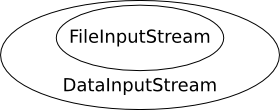
\includegraphics[width=0.6\linewidth]{streams-decorator-pattern.png}
	\caption{Input Stream}
	\label{fig0010}
\end{figure}


\section{Leyendo archivos de texto linea por linea}

El siguiente ejemplo lee el contenido de un archivo de texto linea por linea y lo imprime en la pantalla:


\begin{lstlisting}[language=C++]
int main () {
	// A reference to our file
	var file = File.new_for_path ("data.txt");

	if (!file.query_exists ()) {
		stderr.printf ("File '%s' doesn't exist.\n", file.get_path ());
		return 1;
	}

	try {
		// Open file for reading and wrap returned FileInputStream into a
		// DataInputStream, so we can read line by line
		var dis = new DataInputStream (file.read ());
		string line;
		// Read lines until end of file (null) is reached
		while ((line = dis.read_line (null)) != null) {
			stdout.printf ("%s\n", line);
		}
	} catch (Error e) {
		error ("%s", e.message);
	}

	return 0;
}
\end{lstlisting}

Para compilar y ejecutar este programa se ejecuta en una terminal:
\begin{lstlisting}[language=C++]
$ valac --pkg gio-2.0 gio-sample.vala
$ ./gio-sample
\end{lstlisting}

Es importante puntualizar que no se tiene que cerrar el stream explícitamente. Estos son cerrados automáticamente después de ser ejecutados.

\section{Objetos \textit{\textbf{File}}}


Un objeto \textit{\textbf{File}} es la representación de una ruta a un recurso. Por ejemplo, este puede ser un archivo, o también un directorio. Es importante tener en cuenta que esto no implica nada acerca de la existencia del recurso representado porque el objeto \textit{\textbf{File}} propio no hace operaciones de Entrada/Salida, sólo almacena la ruta. Sin embargo, se puede comprobar la existencia del objeto \textit{\textbf{File}} con el método \textbf{query\_exists ()} :

\begin{lstlisting}[language=C++]
if (file.query_exists ()) {
	// File or directory exists
}
\end{lstlisting}

Para saber si el recurso es un directorio o no se puede buscar el \textit{FileType}:

\begin{lstlisting}[language=C++]
if (file.query_file_type (0) == FileType.DIRECTORY) {
	// It's a directory
}
\end{lstlisting}

Se puede crear un Objeto File desde una ruta de archivo de sistema o una URI:

 
\begin{lstlisting}[language=C++] 
var data_file = File.new_for_path ("data.txt");
var message_of_the_day = File.new_for_path ("/etc/motd");
var home_dir = File.new_for_path (Environment.get_home_dir ());
var web_page = File.new_for_uri ("http://live.gnome.org/Vala");
\end{lstlisting}

Estos son métodos estáticos de fábrica, no constructores, \textbf{\textit{File}} es una interface. Se puede crear una instancia de clases implementando \textbf{\textit{File}}.


GIO trabaja transparentemente a través de varios protocolos. No importa si el acceso es hecho directamente en el sistema local de archivos HTTP, FTP, SFTP, SMB o DAV. Esto es implementado por una capa de sistema de archivo llamado GVFS el cual es diseñado a ser extendible como respaldo de otros protocolos.

\begin{lstlisting}[language=C++]
var home_dir = File.new_for_path (Environment.get_home_dir ());   // ~
var bar_file = home_dir.get_child ("foo").get_child ("bar.txt");  // ~/foo/bar.txt
var foo_dir = bar_file.get_parent ();
\end{lstlisting}

\section{Algunas Operaciones simples de Archivos}

Creando, renombrando, copiando y borrando archivos. Todas las operaciones en esta muestra son no-sincrónicas.

\begin{lstlisting}[language=C++]
int main () {
	try {
		
		// Reference a local file name
		var file = File.new_for_path ("samplefile.txt");
		
		{
			// Create a new file with this name
			var file_stream = file.create (FileCreateFlags.NONE);
			
			// Test for the existence of file
			if (file.query_exists ()) {
				stdout.printf ("File successfully created.\n");
			}
			
			// Write text data to file
			var data_stream = new DataOutputStream (file_stream);
			data_stream.put_string ("Hello, world");
		} // Streams closed at this point
		
		// Determine the size of file as well as other attributes
		var file_info = file.query_info ("*", FileQueryInfoFlags.NONE);
		stdout.printf ("File size: %lld bytes\n", file_info.get_size ());
		stdout.printf ("Content type: %s\n", file_info.get_content_type ());
		
		// Make a copy of file
		var destination = File.new_for_path ("samplefile.bak");
		file.copy (destination, FileCopyFlags.NONE);
		
		// Delete copy
		destination.delete ();
		
		// Rename file
		var renamed = file.set_display_name ("samplefile.data");
		
		// Move file to trash
		renamed.trash ();
		
		stdout.printf ("Everything cleaned up.\n");
		
	} catch (Error e) {
	stderr.printf ("Error: %s\n", e.message);
	return 1;
}

return 0;
}
\end{lstlisting}
 
Compilando y ejecutando

\begin{lstlisting}[language=C++]
$ valac --pkg gio-2.0 gio-file-operations.vala
$ ./gio-file-operations
\end{lstlisting}

\section{Escribiendo Datos}


Este ejemplo crea un archivo de salida, abre un flujo (stream) a ese archivo y escribe algún texto. Para posibles cadenas largas escribe un lazo, el cual checa el número de bytes que han sido escritos, es usado.


\begin{lstlisting}[language=C++]
int main () {
	try {
		// an output file in the current working directory
		var file = File.new_for_path ("out.txt");
		
		// delete if file already exists
		if (file.query_exists ()) {
			file.delete ();
		}
		
		// creating a file and a DataOutputStream to the file
		/*
		Use BufferedOutputStream to increase write speed:
		var dos = new DataOutputStream (new BufferedOutputStream.sized (file.create (FileCreateFlags.REPLACE_DESTINATION), 65536));
		*/
		var dos = new DataOutputStream (file.create (FileCreateFlags.REPLACE_DESTINATION));
		
		// writing a short string to the stream
		dos.put_string ("this is the first line\n");
		
		string text = "this is the second line\n";
		// For long string writes, a loop should be used, because sometimes not all data can be written in one run
		// 'written' is used to check how much of the string has already been written
		uint8[] data = text.data;
		long written = 0;
		while (written < data.length) { 
			// sum of the bytes of 'text' that already have been written to the stream
			written += dos.write (data[written:data.length]);
		}
	} catch (Error e) {
	stderr.printf ("%s\n", e.message);
	return 1;
}

return 0;
}
\end{lstlisting}

Compilar y ejecutar

\begin{lstlisting}[language=C++]
$ valac --pkg gio-2.0 gio-write-data.vala
$ ./gio-write-data
\end{lstlisting}


\section{Leyendo datos binarios}

Esta muestra lee información del archivo de encabezado de imagen BMP así como de la imagen actual de datos.
 
\begin{lstlisting}[language=C++]
int main () {
	try {
		
		// Reference a BMP image file
		var file = File.new_for_uri ("http://wvnvaxa.wvnet.edu/vmswww/images/test8.bmp");
		//      var file = File.new_for_path ("sample.bmp");
		
		// Open file for reading
		var file_stream = file.read ();
		var data_stream = new DataInputStream (file_stream);
		data_stream.set_byte_order (DataStreamByteOrder.LITTLE_ENDIAN);
		
		// Read the signature
		uint16 signature = data_stream.read_uint16 ();
		if (signature != 0x4d42) {   // this hex code means "BM"
			stderr.printf ("Error: %s is not a valid BMP file\n", file.get_basename ());
			return 1;
		}
		
		data_stream.skip (8);        // skip uninteresting data fields
		uint32 image_data_offset = data_stream.read_uint32 ();
		
		data_stream.skip (4);
		uint32 width = data_stream.read_uint32 ();
		uint32 height = data_stream.read_uint32 ();
		
		data_stream.skip (8);
		uint32 image_data_size = data_stream.read_uint32 ();
		
		// Seek and read the image data chunk
		uint8[] buffer = new uint8[image_data_size];
		file_stream.seek (image_data_offset, SeekType.CUR);
		data_stream.read (buffer);
		
		// Show information
		stdout.printf ("Width: %ld px\n", width);
		stdout.printf ("Height: %ld px\n", height);
		stdout.printf ("Image data size: %ld bytes\n", image_data_size);
		
	} catch (Error e) {
	stderr.printf ("Error: %s\n", e.message);
	return 1;
}

return 0;
}
\end{lstlisting}

Compilar y ejecutar

\begin{lstlisting}[language=C++]
$ valac --pkg gio-2.0 gio-binary-sample.vala 
$ ./gio-binary-sample
\end{lstlisting}


\section{Listando el contenido del directorio}

\begin{lstlisting}[language=C++]
int main (string[] args) {
	try {
		var directory = File.new_for_path (".");
		
		if (args.length > 1) {
			directory = File.new_for_commandline_arg (args[1]);
		}
		
		var enumerator = directory.enumerate_children (FileAttribute.STANDARD_NAME, 0);
		
		FileInfo file_info;
		while ((file_info = enumerator.next_file ()) != null) {
			stdout.printf ("%s\n", file_info.get_name ());
		}
		
	} catch (Error e) {
	stderr.printf ("Error: %s\n", e.message);
	return 1;
}

return 0;
}
\end{lstlisting}

Compilar y ejecutar

\begin{lstlisting}[language=C++]
$ valac --pkg gio-2.0 gio-ls.vala
$ ./gio-ls
\end{lstlisting}

\section{Listado de Archivos Asíncronos}


\begin{lstlisting}[language=C++]
using Gtk;

/**
* Loads the list of files in user's home directory and displays them
* in a GTK+ list view.
*/
class ASyncGIOSample : Window {
	
	private ListStore model;
	
	public ASyncGIOSample () {
		
		// Set up the window
		set_default_size (300, 200);
		this.destroy.connect (Gtk.main_quit);
		
		// Set up the list widget and its model
		this.model = new ListStore (1, typeof (string));
		var list = new TreeView.with_model (this.model);
		list.insert_column_with_attributes (-1, "Filename",
		new CellRendererText (), "text", 0);
		
		// Put list widget into a scrollable area and add it to the window
		var scroll = new ScrolledWindow (null, null);
		scroll.set_policy (PolicyType.NEVER, PolicyType.AUTOMATIC);
		scroll.add (list);
		add (scroll);
		
		// start file listing process
		list_directory.begin ();
	}
	
	private async void list_directory () {
		stdout.printf ("Start scanning home directory\n");
		var dir = File.new_for_path (Environment.get_home_dir ());
		try {
			// asynchronous call, to get directory entries
			var e = yield dir.enumerate_children_async (FileAttribute.STANDARD_NAME,
			0, Priority.DEFAULT);
			while (true) {
				// asynchronous call, to get entries so far
				var files = yield e.next_files_async (10, Priority.DEFAULT);
				if (files == null) {
					break;
				}
				// append the files found so far to the list
				foreach (var info in files) {
					TreeIter iter;
					this.model.append (out iter);
					this.model.set (iter, 0, info.get_name ());
				}
			}
		} catch (Error err) {
		stderr.printf ("Error: list_files failed: %s\n", err.message);
	}
}

static int main (string[] args) {
	Gtk.init (ref args);
	
	var demo = new ASyncGIOSample ();
	demo.show_all ();
	
	Gtk.main ();
	return 0;
}
}
\end{lstlisting}

Compilar y ejecutar

\begin{lstlisting}[language=C++]
$ valac --pkg gtk+-3.0 gio-async.vala
$ ./gio-async
\end{lstlisting}


\section{Flujo de lectura asíncrona}


\begin{lstlisting}[language=C++]
MainLoop main_loop;

async void read_something_async (File file) {
	var text = new StringBuilder ();
	print ("Start...\n");
	
	try {
		var dis = new DataInputStream (file.read ());
		string line = null;
		while ((line = yield dis.read_line_async (Priority.DEFAULT)) != null) {
			text.append (line);
			text.append_c ('\n');
		}
		print (text.str);
	} catch (Error e) {
	error (e.message);
}
main_loop.quit ();
}

void main (string[] args) {
	
	var file = File.new_for_uri ("http://www.gnome.org");
	
	if (args.length > 1) {
		file = File.new_for_commandline_arg (args[1]);
	}
	
	main_loop = new MainLoop ();
	read_something_async (file);
	main_loop.run ();
}
\end{lstlisting}

Compilar y ejecutar

\begin{lstlisting}[language=C++]
$ valac --pkg gio-2.0 gio-async-reading.vala
$ ./gio-async-reading
\end{lstlisting}


\chapter{Programación con GTK+}

En términos de ingeniería del software, un widget es un componente software visible y personalizable. Visible porque está pensado para ser usado en los interfaces gráficos de los programas, y personalizable porque el programador puede cambiar muchas de sus propiedades. De esta forma se logra una gran reutilización del software, un objetivo prioritario en ingeniería del software. Los widgtes se combinan para construir los interfaces gráficos de usuario. El programador los adapta según sus necesidades sin tener que escribir más código que el necesario para definir los nuevos valores de las propiedades de los widgets.

La librería GTK+ sigue el modelo de programación orientado a objetos. La jerarquía de objetos comienza en GObject de la librería Glib del que hereda GtkObject. Todos los widgets heredan de la clase de objetos GtkWidget, que a su vez hereda directamente de GtkObject. La clase GtkWidget contiene las propiedades comunes a todos los widgets; cada widget particular le añade sus propias propiedades.

Los widgets se definen mediante punteros a una estructura GtkWidget. En GTK+, los widgets presentan una relación padre/hijo entre sí. 
Las aplicaciones suelen tener un widget \textbf{ventana} de nivel superior que no tiene padre, pero aparte de él, todos los widgets que se usen en una aplicación deberán tener un widget padre. Al widget padre se le denomina contenedor. El proceso de creación de un widget consta de dos pasos: el de creación propiamente dicho y el de visualización. La función de creación de un widget tiene un nombre que sigue el esquema gtk\_nombre\_new donde \textbf{nombre} debe sustituirse por el nombre del widget que se desea crear. La función gtk\_widget\_show hará visible el widget creado.

La función de creación de un widget gtk\_nombre\_new devuelve un puntero a un objeto de tipo GtkWidget y no un puntero a un widget del tipo creado. Por ejemplo, la función gtk\_button\_new devuelve un puntero a un objeto de GtkWidget y no una referencia a un botón. Esta referencia puede convertirse a una referencia a un objeto GtkButton mediante la macro GTK\_BUTTON, si se desea utilizar en lugares donde se requieran objetos botones. Aunque sería posible pasar en esos casos la referencia genérica, el compilador se quejará si se hace así posibilitando un control de tipos de objetos. Todo widget tiene una macro de conversión de una referencia genérica a una referencia al tipo propio. Eso sí, la macro únicamente funcionará correctamente si el widget referenciado fue creado con la función de creación del tipo apropiado, lo que incluye el propio tipo del widget o un descendiente.

El interfaz gráfico de una aplicación se construye combinando diferentes widgets (ventanas, cuadros combinados, cuadros de texto, botones, ...) y se establecen diversas retrollamadas (callbacks) para estos widgets, de esta forma se obtiene el procesamiento requerido por el programa a medida que se producen ciertas señales que a su vez provocan las retrollamadas. Las señales se producen por diversos sucesos como oprimir el boton de un ratón que se encuentra sobre un widget botón, pasar el cursor por encima de un widget u oprimir una tecla.

GTK+ utiliza GDK para visualizar los widgets. GDK es una interfaz de programación (API) de aplicaciones que se situa por encima de la API gráfica nativa como Xlib o Win32. De esta forma portando GDK pueden utilizarse las aplicaciones construidas con GTK+ en otras plataformas. 

GTK+ o The GIMP Toolkit es un conjunto de bibliotecas multiplataforma para desarrollar interfaces gráficas de usuario (GUI), principalmente para los entornos gráficos GNOME, XFCE y ROX aunque también se puede usar en el escritorio de Windows, Mac OS y otros.

Inicialmente fueron creadas para desarrollar el programa de edición de imagen GIMP, sin embargo actualmente se usan bastante por muchos otros programas en los sistemas GNU/Linux. Junto a Qt es una de las bibliotecas más populares para Wayland y X Window System.

Licenciado bajo los términos de LGPL, GTK+ permite la creación de tanto software libre como software propietario. GTK+ es parte del proyecto GNU.

GTK+ se basa en varias bibliotecas desarrolladas por el equipo de GTK+ y de GNOME:

\begin{itemize}
\item \textbf{GLib} Biblioteca de bajo nivel estructura básica de GTK+ y GNOME. Proporciona manejo de estructura de datos para C, portabilidad, interfaces para funcionalidades de tiempo de ejecución como ciclos, hilos, carga dinámica o un sistema de objetos.

\item \textbf{GTK} Biblioteca que actúa como intermediario entre gráficos de bajo nivel y gráficos de alto nivel.

\item \textbf{ATK} Biblioteca para crear interfaces con características de una gran accesibilidad muy importante para personas discapacitadas o minusválidos. Pueden usarse utilerías como lupas de aumento, lectores de pantalla, o entradas de datos alternativas al clásico teclado o ratón.

\item \textbf{Pango} Biblioteca para el diseño y renderizado de texto, hace hincapié especialmente en la internacionalización. Es el núcleo para manejar las fuentes y el texto de GTK+2.

\item \textbf{Cairo}  Biblioteca de renderizado avanzado de controles de aplicación. 

\end{itemize}

\section{Ejemplo Básico}

En el siguiente ejemplo se muestra el programa gráfico que despliega un boton. Y al pulsarlo cambia la etiqueta de un botón.

\begin{lstlisting}[language=C++]
using Gtk;

int main (string[] args) {
    Gtk.init (ref args);

    var window = new Window ();
    window.title = "Primer Programa GTK+";
    window.border_width = 10;
    window.window_position = WindowPosition.CENTER;
    window.set_default_size (350, 70);
    window.destroy.connect (Gtk.main_quit);

    var button = new Button.with_label ("Pulsame!");
    button.clicked.connect (() => {
        button.label = "Gracias";
    });

    window.add (button);
    window.show_all ();

    Gtk.main ();
    return 0;
}

\end{lstlisting}

para compilar el programa se debe ejecutar:

\begin{lstlisting}[language=C++]
$ valac --pkg gtk+-3.0 gtk-hello.vala
$ ./gtk-hello
\end{lstlisting}

\section{Sincronización de Widgets}

En la siguiente aplicación se sincronizan dos widgets:

\begin{lstlisting}[language=C++]
using Gtk;

public class SyncSample : Window {

    private SpinButton spin_box;
    private Scale slider;

    public SyncSample () {
        this.title = "Introduce tu edad";
        this.window_position = WindowPosition.CENTER;
        this.destroy.connect (Gtk.main_quit);
        set_default_size (300, 20);

        spin_box = new SpinButton.with_range (0, 130, 1);
        slider = new Scale.with_range (Orientation.HORIZONTAL, 0, 130, 1);
        spin_box.adjustment.value_changed.connect (() => {
            slider.adjustment.value = spin_box.adjustment.value;
        });
        slider.adjustment.value_changed.connect (() => {
            spin_box.adjustment.value = slider.adjustment.value;
        });
        spin_box.adjustment.value = 35;

        var hbox = new Box (Orientation.HORIZONTAL, 5);
        hbox.homogeneous = true;
        hbox.add (spin_box);
        hbox.add (slider);
        add (hbox);
    }

    public static int main (string[] args) {
        Gtk.init (ref args);

        var window = new SyncSample ();
        window.show_all ();

        Gtk.main ();
        return 0;
    }
}
\end{lstlisting}

\begin{lstlisting}[language=C++]
$ valac --pkg gtk+-3.0 gtk-sync-sample.vala
$ ./gtk-sync-sample
\end{lstlisting}

\section{Temporizador}

El siguiente programa dispara una función de contador cada segundo

\begin{lstlisting}[language=C++]
public class Sample : Object
{
	public static int conta;
   private static bool task()
   {
      stdout.printf("Ya %g \n", conta);
      stdout.flush();
  	 conta++;    
      if (conta<=10) {
		 return true; // false para terminar el temporizador
		 }
	else {
		return false;
	}
   }

   public static int main(string[] args)
   {
	   conta=0;
      Timeout.add_seconds(1, task);
      new MainLoop().run();
      return 0;
   }
}
\end{lstlisting}

El diseño del temporizador es muy importante para muchos proyectos cuya lectura es periódica ya sea esta lectura de información del usuario o de sensores, la clave del funcionamiento esta en la instrucción \textbf{timeout}, la cual configura, en este ejemplo, la función \textbf{task} para que se realice periódicamente en intervalos de un segundo.

Para compilar el programa se ejecuta el siguiente código:

\begin{lstlisting}[language=C++]
$ valac temporizador.vala
$ ./temporizador
\end{lstlisting}

una aplicación interesante del temporizador es el diseño de un reloj.

\subsection{Proyecto de Ejemplo: Diseñando un reloj}

Para aplicar los conocimientos del temporizador se plantea el diseño de un reloj, para ello en el programa de glade se diseña la interface

\begin{figure}
	\centering
	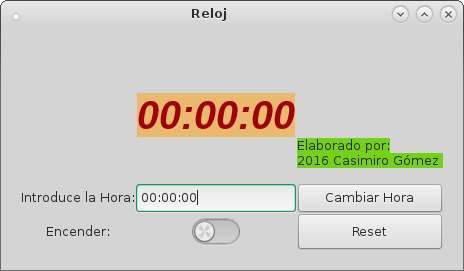
\includegraphics[width=0.9\linewidth]{reloj.png}
	\caption{Pantalla del reloj diseñada en Glade}
	\label{fig0011}
\end{figure}
En la figura \ref{fig0020} se muestran los widgets usados en el diseño de la pantalla del reloj usando el programa Glade. El diseño en Glade debe seguir cierto orden:

\begin{itemize}
\item 1.- Primero debe colocarse un contenedor, en este caso el contenedor usado es \textbf{Window} (ventana en español), a este contenedor se le deja el nombre de \textbf{window1} que aparece por defecto, en la figura \ref{fig0020} se observa el nombre como \textbf{GtkWindow}.
\item 2.- Colocar la rejilla, en este caso se coloca una rejilla de $3X3$ a la cual se le deja el nombre por defecto \textbf{grid1}, en la figura \ref{fig0020} aparece como \textbf{GtkGrid}.
\item 3.- Se colocan tres etiquetas (o Label en inglés) las cuales se nombran \textbf{reloj}, \textbf{IntroHora} y \textbf{Encender}. La etiqueta de reloj desplegará la hora con el formato HH:MM:SS y se actualizará cada segundo, las otras dos son solo etiquetas que desplegarán mensajes para entrada de datos y boton interruptor respectivamente.
\item 4.- Se colocan dos botones, el botón de \textbf{bReset} y el boton de \textbf{bCambiar}. El botón de \emph{bReset} reiniciará el reloj al valor \textbf{00:00:00} y el boton de \emph{bCambiar} cambiara el valor del reloj al valor que el usuario introduzca en la entrada de datos \textbf{GtkEntry} llamada \textbf{ValorHora}.
\item 5.- Se coloca una entrada de datos \textbf{GtkEntry} llamada \textbf{ValorHora}, en donde el usuario introducirá la corrección de hora del reloj y posteriormente la enviará cuando pulse el botón \textbf{bCambiar}.

\end{itemize}


\begin{figure}
	\centering
	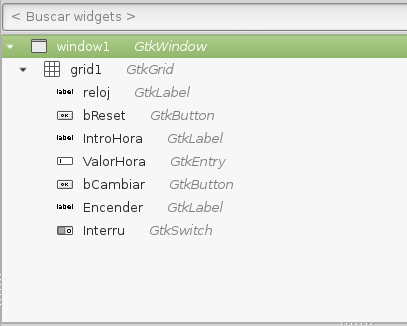
\includegraphics[width=0.7\linewidth]{widgetReloj.png}
	\caption{Widget usados en el diseño de la Pantalla del reloj en Glade}
	\label{fig0020}
\end{figure}


Una vez terminado el diseño de la pantalla en Glade, se configuran las funciones que controlarán los botones, como se puede observa en las figuras \ref{fig0021}, \ref{fig0022}, y \ref{fig0023}. En este caso se necesitan tres funciones manejadoras, dos para los botones \textbf{bCambiar} y \textbf{bReset}, y una para el boton interruptor \textbf{Interru}. Las funciones manejadoras para el boton \textbf{bCambiar}, \textbf{bReset} y   \textbf{Interru} se definen en la propiedades de sus respectivos botones en las pestaña de señales se especifica el nombre de la función manipuladora. Como se puede observar cuando se da click sobre el manipulador y se escribe una \textbf{o} el mismo glade propone un nombre a la función, es recomendable utilizar el nombre de la función propuesta y adicionar el \textit{namespace} y la \textit{clase} al nombre de la función manipuladora, estos nombres se escriben en minúscula aún cuando el nombre del namespace y de la clase sean en mayúsculas. En el caso del botón \emph{Interru}, el nombre propuesto fue \textbf{on\_Interru\_state\_set} y al adicionar el \textit{namespace} y la \textit{clase} el nombre queda \textbf{beagle\_control\_on\_Interru\_state\_set}

\begin{figure}
	\centering
	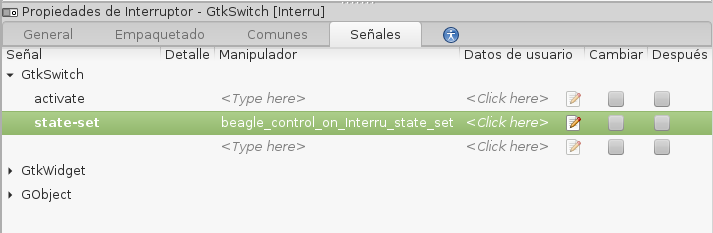
\includegraphics[width=0.8\linewidth]{Interru.png}
	\caption{Manipulador del botón Interruptor}
	\label{fig0021}
\end{figure}

\begin{figure}
	\centering
	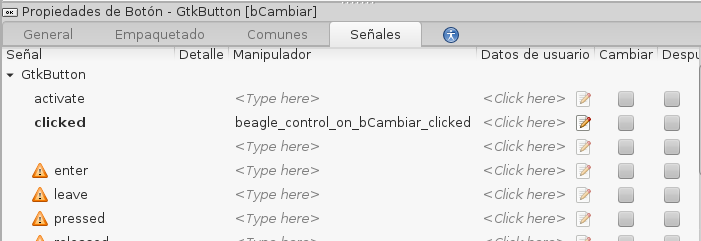
\includegraphics[width=0.8\linewidth]{bCambiar.png}
	\caption{Manipulador del botón bCambiar}
	\label{fig0022}
\end{figure}

\begin{figure}
	\centering
	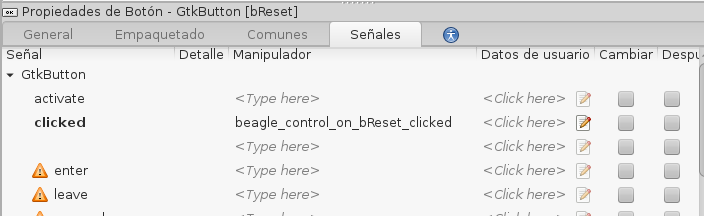
\includegraphics[width=0.8\linewidth]{bReset.png}
	\caption{Manipulador del botón bReset}
	\label{fig0023}
\end{figure}

Para el botón bReset el código es el siguiente:

\begin{lstlisting}[language=C++]
	[CCode ( instance_pos = -1) ]
  	public void  on_bReset_clicked ( Button source ) {
		Useg=-1;
		Dseg=0;
		Umin=0;
		Dmin=0;
		Uhora=0;
		Dhora=0;
	}
\end{lstlisting}


Como se muestra se inicializan las variables del reloj, cada variable esta dividida en segundo, minutos y horas y cada una respectivamente tiene sus unidades y sus decenas, de tal forma que la variable de unidades de segundos se llama Useg y cuenta del 0 al 9 y la variable de decenas de segundos cuenta del 0 al 5 y se llama Dseg. En el caso de los minutos es la misma técnica. Para las horas solo hay que tomar en cuenta que el límite son las 23 horas, si llegar a las 24 horas. Estas variables deben ser modificadas en cualquier método de la clase y actualizarse por lo cual se deben definir como varibales globales, como se muestra en el siguiente código

\begin{lstlisting}[language=C++]
using Gtk ;

 namespace Beagle {
  	public class Control:Object {
	
	public string texto = "";
	public static Entry entrada;
	public static Label reloj;
	public static bool bandera;

    public static int Useg;
    public static int Dseg;
    public static int Umin;
    public static int Dmin;
    public static int Uhora;
    public static int Dhora;
    public static string hora;
\end{lstlisting}


La variable hora también es una variable global que es una cadena, esta cadena es resultada de la conversión y concatenación de las variables de cuenta Useg, Dseg, Umin, Dmin, Uhora y Dhora. Y es la que se imprime. Las variables entrada y reloj asimismo son variables globales que tomaran la entrada de datos del glade y permitirán la impresión de valores del reloj (en este caso de la varible hora) y la captura de hora que introduzca el usuario permitiendo su acceso en cualquier parte de la clase.

En el siguiente código se muestra la función manipuladora del botón bCambiar

\begin{lstlisting}[language=C++]	
	[CCode ( instance_pos = -1) ]
  	public void  on_bCambiar_clicked ( Button source ) {
		texto= entrada.get_text();
		 Dhora=int.parse(texto[0:1]);
		 Uhora=int.parse(texto[1:2]);
		 Dmin=int.parse(texto[3:4]);
		 Umin=int.parse(texto[4:5]);
		 Dseg=int.parse(texto[6:7]);
		 Useg=int.parse(texto[7:8]);		 
		reloj.set_text(texto);
		stdout.printf("Hola Mundo %s oj \n", texto );
	}
\end{lstlisting}



\section{Programa Usando Hilos}

Un programa escrito en Vala puede tener más de un hilo en ejecución, permitiendole hacer más de una cosa al mismo tiempo. Fuera del ámbito de Vala los hilos comparten un mismo procesador o no, dependiendo del entorno de ejecución.

Un hilo en Vala no se define en el tiempo de compilación, en lugar de eso se define una porción del código Vala para que se ejecute como un nuevo hilo. Esto se realiza mediante el método estático de la clase Thread de la biblioteca GLib, como puede verse en siguiente ejemplo:


\begin{lstlisting}[language=C++]
public class MyThread : Object {
	public int x_times { get; private set; }

	public MyThread (int times) {
		this.x_times = times;
	}

	public int run () {
		for (int i = 0; i < this.x_times; i++) {
			stdout.printf ("ping! %d/%d\n", i + 1, this.x_times);
			Thread.usleep (10000);
		}

		// return & exit have the same effect
		return 43;
	}
}

public static int main (string[] args) {
	// Check whether threads are supported:
	if (Thread.supported () == false) {
		stderr.printf ("Threads are not supported!\n");
		return -1;
	}

	try {
		// Start a thread:
		MyThread my_thread = new MyThread (10);
		Thread<int> thread = new Thread<int>.try ("My fst. thread", my_thread.run);

		// Wait until thread finishes:
		int result = thread.join ();
		// Output: `Thread stopped! Return value: 42`
		stdout.printf ("Thread stopped! Return value: %d\n", result);
	} catch (Error e) {
		stdout.printf ("Error: %s\n", e.message);
	}

	return 0;
}

\end{lstlisting}

\section{Dos hilos}


\begin{lstlisting}[language=C++]
class MyThread {

    private string name;
    private int count = 0;

    public MyThread (string name) {
        this.name = name;
    }

    public void* thread_func () {
        while (true) {
            stdout.printf ("%s: %i\n", this.name, this.count);
            this.count++;
            Thread.usleep (Random.int_range (0, 200000));
        }
    }
}

int main () {
    if (!Thread.supported ()) {
        stderr.printf ("Cannot run without thread support.\n");
        return 1;
    }

    var thread_a_data = new MyThread ("A");
    var thread_b_data = new MyThread ("B");

    try {
        // Start two threads
        /* With error handling */
        Thread<void*> thread_a = new Thread<void*>.try ("thread_a", thread_a_data.thread_func);
        /* Without error handling (is not using the try/catch) */
        Thread<void*> thread_b = new Thread<void*> ("thread_b", thread_b_data.thread_func);

        // Wait for threads to finish (this will never happen in our case, but anyway)
        thread_a.join ();
        thread_b.join ();

    } catch (Error e) {
        stderr.printf ("%s\n", e.message);
        return 1;
    }


    return 0;
}
\end{lstlisting}
 
\chapter{Controlando linux desde Vala}

La manera de la que vamos a acceder a los GPIO (en este caso al 17) es como si fuesen directorios. Podemos utilizar comandos como \textbf{ls}, \textbf{cat} o \textbf{echo}, entre otros, para conocer la estructura y contenidos de los directorios. 

Ahora mismo no tenemos ningún pin accesible. Ni de entrada ni de salida. Tenemos que crearlo nosotros mismos. Queremos tener acceso al GPIO 17, así que introducimos el siguiente comando: 

\begin{lstlisting}[language=bash]
echo 17 > /sys/class/gpio/export
\end{lstlisting}

Tras esto, el sistema ha creado un archivo con una estructura GPIO que corresponde al número 17. A continuación, tenemos que informar a la Raspberry Pi de si el pin va a ser de salida o de entrada. Como lo que queremos es encender un LED, el GPIO 17 será de salida. Introducimos el siguiente comando: 

\begin{lstlisting}[language=bash]
echo out > /sys/class/gpio/gpio17/direction
\end{lstlisting}


Con esto, el sistema ya sabe que el pin será de salida. Ahora tendremos que darle valores. Existen dos posibles: \textbf{0} y \textbf{1}. 

\subsection{Para encender el LED}

\begin{lstlisting}[language=bash]
echo 1 > /sys/class/gpio/gpio17/value
\end{lstlisting}


 \subsection{ Para apagar el LED:}
 
 \begin{lstlisting}[language=bash]
echo 0 > /sys/class/gpio/gpio17/value
\end{lstlisting}

Una vez hayamos acabado de encender y apagar el LED, tendremos que eliminar la entrada GPIO creada, es decir, el GPIO 17. Para ello introduciremos el siguiente comando: 

\begin{lstlisting}[language=bash]	
echo 17 > /sys/class/gpio/unexport
\end{lstlisting}


\section{Programación serial con Vala}

En Linux, los periféricos se encuentran representados como simples ficheros del
sistema de archivos. De esta forma, si se quiere enviar datos a través del puerto
serie, basta con abrir el fichero asociado al puerto y escribir con las funciones de
siempre. Cada uno de los puertos serie tiene asociado uno o más ficheros de
dispositivo. En la Tabla \ref{T001} se muestra la asociación más habitual entre los
puertos serie y los ficheros del sistema de archivos.

\begin{table}[htbp]
\begin{center}
\begin{tabular}{|l|l|}
\hline
Puerto & Archivo \\
\hline \hline
COM1 & /dev/ttyS0 \\ \hline
COM2 & /dev/ttyS1 \\ \hline
COM3 & /dev/ttyS2 \\ \hline
\end{tabular}
\caption{Asociación de Puertos Seriales a archivos.}
\label{T001}
\end{center}
\end{table}

Para acceder al puerto únicamente es necesario abrir el fichero asociado
mediante la llamada al sistema \emph{open}. Se debe tener en cuenta que, en Linux, los
ficheros asociados a los dispositivos no suelen tener permiso de acceso para los
usuarios. Para evitar este problema existen varias soluciones:

\begin{itemize}
\item Cambiar los permisos del fichero/s asociado al dispositivo y dar permisos
de lectura y escritura a los usuarios.
\item Ejecutar el programa realizado en modo super-usuario (root).
\end{itemize}

La especificación de la función open es la siguiente:
\begin{lstlisting}[language=bash]	
int handle = Posix.open ("/dev/ttyS1", Posix.O_RDWR | Posix.O_NOCTTY | O_NDELAY);
\end{lstlisting}

Se debe indicar el fichero que se desea abrir y las opciones de apertura
necesarias. Estas opciones se indican mediante el uso de constantes definidas
por el operativo. La función retorna un número
negativo si no se pudo abrir el fichero indicado. Si el fichero se abrió
correctamente, se retorna un descriptor de fichero (un entero no negativo que se
utiliza en las operaciones de E/S posteriores, como en read, write, etc.).

En el código se muestra el uso de la llamada al sistema open.
La opción O\_RDWR indica que el fichero /dev/ttyS1 (fichero asociado al puerto
COM2) se debe abrir en modo lectura y escritura.
La opción O\_NOCTTY indica que el fichero no se abrirá como controlador de
terminal tty. Si no se especifica esta opción una señal de finalización (abort)
enviada por la línea finalizaría la ejecución.

Para mandar datos al puerto se emplea la llamada al sistema write:

\begin{lstlisting}[language=bash]
int l = (int)Posix.write (handle, data, data.length);
\end{lstlisting}

Escribe hasta \emph{data.length} bytes en el fichero referenciado por el descriptor de fichero \emph{handle}
desde el búfer que comienza en data.

Para leer datos del puerto se emplea la llamada al sistema read:
\begin{lstlisting}[language=bash]
int bytesRead=(int)Posix.read(m_fd, m_buf, max_buf_size);
\end{lstlisting}

Intenta leer hasta \emph{max\_buf\_size} bytes del fichero cuyo descriptor de fichero es 
\emph{m\_fd} y guardarlos en la zona de memoria que empieza en \emph{m\_buf}. En el código anterios se puede ver una forma de uso. La llamada al sistema \emph{read}, no finaliza el buffer
donde deposita los datos con el ASCII nulo. Es por ello, que esta tarea se hace
explícitamente: 
\begin{lstlisting}[language=bash]
buffer[leo]='\0'; . 
\end{lstlisting}

\subsection{Conceptos de entrada para dispositivos serie}

Hay tres conceptos diferentes de entrada para dispositivos serie. Según la
aplicación que se quiera realizar se debe escoger el concepto apropiado. Siempre
que sea posible, se recomienda no obtener una cadena completa mediante un
ciclo que vaya leyendo carácter a carácter.

\subsubsection{Proceso de entrada canónico}

Es el modo de proceso normal para terminales, pero puede ser útil también para
comunicaciones con otros dispositivos. Toda la entrada es procesada en unidades
de líneas, lo que significa que un read sólo devolverá una línea completa de
entrada. Una línea, por defecto, está finalizada con un NL y fin de fichero o con
un carácter fin de línea. Un CR (el fin de línea por defecto en DOS/Windows) no
terminará una línea con la configuración por defecto.
El proceso de entrada canónica también puede manejar los caracteres borrado,
borrado de palabra, reimprimir carácter, traducir CR a NL, etc.

\subsubsection{Proceso de entrada no canónico}

Maneja un número fijo de caracteres por lectura y permite un carácter
temporizador. Este modo se debería usar si la aplicación siempre lee un número
fijo de caracteres o si el dispositivo conectado envía ráfagas de caracteres.


\subsubsection{Entrada asíncrona}


Los dos procesos de entrada descritos anteriormente se pueden usar en dos
modos:

\begin{itemize}
\item \textbf{Modo síncrono}: la sentencia read se bloqueará hasta que la lectura esté
completa (este es el modo por defecto).

\item \textbf{Modo asíncrono}: la sentencia read devolverá inmediatamente y enviará
una señal al programa llamador cuando esté completa. Esta señal puede
ser recibida por un manejador de señales que la tratará adecuadamente.
\end{itemize}

\subsubsection{Espera de entradas de origen múltiple}

No es un modo diferente de entrada, pero puede ser útil si se están manejando
dispositivos múltiples. En aplicaciones donde se esperen entradas de distintos
orígenes, se procesarán aquellas entradas que estén disponibles y, una vez
procesadas, se esperará la llegada de nuevas entradas.

\subsection{Configuración del puerto serie en Linux}

En esta sección se mostrará la configuración del puerto serie en lenguaje Vala
utilizando la interfaz que proporciona el estándar POSIX (acrónimo de Portable
operating system interface). La información aquí mostrada se ha obtenido, entre
otras fuentes, del documento ``Serial Programming Guide for POSIX Operating
Systems''.
En el archivo de cabecera <termios.h> se definen las estructuras y funciones
necesarias para llevar a cabo la configuración del puerto serie. La estructura más
importante es la estructura termios formada por los miembros mostrados en la
Tabla \ref{T002}.

\begin{table}[htbp]
\begin{center}
\begin{tabular}{|l|l|}
\hline
Miembro & Descripción \\
\hline \hline
c\_cflag & Opciones de control \\ \hline
c\_lflag & Opciones locales \\ \hline
c\_iflag & Opciones de entrada \\ \hline
c\_oflag & Opciones de salida \\ \hline
c\_cc & Caracteres de control \\ \hline
c\_ispeed & Velocidad (baudios) de entrada\\ \hline
c\_ospeed & Velocidad (baudios) de salida \\ \hline
\end{tabular}
\caption{Miembros de la estructura termios}
\label{T002}
\end{center}
\end{table}

Las funciones que se utilizarán para llevar a cabo la configuración del puerto
serie son:

\begin{itemize}
\item tcgetattr: Se utiliza para obtener los parámetros actuales del puerto.
\begin{lstlisting}[language=bash]
int tcgetattr ( int fd, struct termios *termios_p );
\end{lstlisting}

Obtiene los parámetros asociados con el objeto referido por fd y los
guarda en la estructura termios referenciada por termios\_p.

\item tcsetattr: Se utiliza para actualizar los parámetros del puerto.

\begin{lstlisting}[language=bash]
int tcsetattr ( int fd, int optional_actions, struct termios *termios_p);
\end{lstlisting}

Establece los parámetros de la terminal con descriptor de fichero fd, desde
la estructura termios referenciada por termios\_p. El argumento
optional\_actions especifica cuándo tienen efecto los cambios:
\begin{itemize}
	\item TCSANOW: El cambio ocurre inmediatamente.
	\item TCSADRAIN: El cambio ocurre después de que toda la salida escrita a
fd haya sido transmitida. Esta función debería emplearse cuando se
cambien parámetros que afecten a la salida.
	\item TCSAFLUSH: El cambio ocurre después de que toda la salida escrita
al objeto referenciado por fd haya sido transmitida, y toda la entrada
que se haya recibido pero no leído será descartada antes de que se
haga el cambio.
\end{itemize}
\item tcflush: Se utiliza para vaciar los buffers de entrada/salida.

\begin{lstlisting}[language=bash]
int tcsetattr ( int fd, int optional_actions, struct termios *termios_p);
\end{lstlisting}

Descarta datos escritos al objeto referido por fd pero no transmitidos, o
datos recibidos pero no leídos, dependiendo del valor de queue\_selector:

\begin{itemize}
\item TCIFLUSH: Vuelca datos recibidos pero no leídos.
\item TCOFLUSH: Vuelca datos escritos pero no transmitidos.
\item TCIOFLUSH: Vuelca tanto los datos recibidos pero no leídos, como los
escritos pero no transmitidos.
\end{itemize}
\item cfsetospeed: Se utiliza para establecer la velocidad de salida.

\begin{lstlisting}[language=bash]
int cfsetospeed ( struct termios *termios_p, speed_t speed );
\end{lstlisting}
Establece la velocidad de salida, guardada en la estructura termios
apuntada por termios\_p, a speed, que debe ser una de estas constantes:
B0, B50, B75, B110, B134, B150, B200, B300, B600, B1200, B1800,
B2400, B4800, B9600, B19200, B38400, B57600, B115200, B230400.
Los nuevos valores no hacen efecto hasta que se llame con éxito a
tcsetattr().

\item cfsetispeed: Se utiliza para establecer la velocidad de entrada.

\begin{lstlisting}[language=bash]
int cfsetispeed ( struct termios *termios_p, speed_t speed );
\end{lstlisting}
Establece la velocidad de entrada, guardada en la estructura termios
apuntada por termios\_p, a speed, que debe ser una de estas constantes:
B0, B50, B75, B110, B134, B150, B200, B300, B600, B1200, B1800,
B2400, B4800, B9600, B19200, B38400, B57600, B115200, B230400.
Si la velocidad de entrada se pone a cero, entonces será igual a la de
salida. Los nuevos valores no hacen efecto hasta que se llame con éxito a
tcsetattr().
\end{itemize}
En el siguiente ejemplo se puede ver un fragmento de código que muestra la
utilización de alguna de las funciones comentadas.






\bibliographystyle{acm}
\bibliography{../bibliografia}

\end{document}